\chapter{Lý thuyết tính toán}
\minitoc
\vspace{0.5cm}

% Trong chương này ta sẽ xem xét cơ sở lý thuyết của khoa học máy tính. Theo một nghĩa nào
% đó, nội dung trong chương này đưa khoa học máy tính lên vị thế của một nghành khoa học
% chính xác. Mặc dù chúng có vẻ hơi trừu tượng, nhưng những kiến thức này có rất nhiều ứng
% dụng thực tế. Đặc biệt, chúng ta sẽ khám phá các kết quả liên quan đến khả năng của các
% ngôn ngữ lập trình và giải thích cách mà các hệ thống mã hoá hiện nay được sử dụng trong
% giao tiếp trên Internet.

%
\noindent
Trong chương này ta xem xét câu hỏi liên quan đến việc máy tính có thể hay không thể làm
gì. Ta sẽ mô tả một máy đơn giản, gọi là máy Turing, như một công cụ để xác định biên giới
giữa các bài toán có thể và các bài toán không thể giải được bằng máy tính. Sau đó, ta
giới thiệu một bài toán đặc biệt, gọi là bài toán dừng, và chứng minh rằng việc giải nó là
nằm ngoài khả năng của mọi hệ thống tính toán. Cuối cùng ta chỉ ra rằng, trong số các bài
toán có thể giải bằng máy tính về mặt lý thuyết, có tồn tại những bài toán phức tạp đến
mức không giải được trên thực tế.

\section{Các hàm và tính toán}
Trước khi thảo luận về khả năng của máy tính, ta môt tả mối liên hệ giữa giải quyết bài
toán và tính toán hàm.

Một \textit{hàm} theo nghĩa toán học là một tương ứng giữa một tập các giá trị đầu vào và
một tập các giá trị đầu ra sao cho với mỗi đầu vào ta chỉ có tương ứng một đầu ra duy
nhất. Một ví dụ là hàm là chuyển đơn vị yard thành mét. Ở đây, mỗi giá trị tính theo yard
được đặt tương ứng với một giá trị tính theo mét và hai giá trị này phải phản ánh cùng một
độ dài. Một ví dụ khác là hàm sắp xếp, nó gắn mỗi danh sách các giá trị số đầu vào với một
danh sách các giá trị số đầu ra chính là dãy đầu vào nhưng đã được sắp xếp theo chiều tăng
dần. Một ví dụ khác nữa là hàm cộng, nó gắn một cặp giá trị số đầu vào với một giá trị đầu
ra là tổng của cặp số đó.

Quá trình xác định các giá trị đầu ra cụ thể tương ứng với giá trị đầu vào được gọi là
\textit{việc tính toán các hàm}. Khả năng tính toán các hàm là quan trong bởi vì chính
cách tính toán các hàm mà ta có thể giải quyết các bài toán. Ví dụ, để giải bài toán cộng,
ta phải tính toán hàm cộng; để sắp xếp một danh sách, ta phải tính toán hàm sắp xếp. Theo
cách này, một nhiệm vụ cơ bản của khoa học máy tính là tìm cách tính toán các hàm liên
quan đến bài toán mà ta muốn giải quyết.

Ta xem xét, ví dụ, một hệ thống tính hàm trong đó các đầu vào và đầu ra của hàm có thể
được xác định trước và ghi trong một bảng. Mỗi khi cần tính đầu vào của hàm, ta chỉ cần
tìm vị trí đầu vào ở trong bảng và ở vị trí tương ứng ta tìm thấy đầu ra. Bởi vậy việc
tính toán các hàm được rút gọn thành quá trình tìm kiếm trong bảng. Các hệ thống kiểu này
tiện lợi nhưng bị giới hạn do có nhiều hàm không thể được biểu diễn đầy đủ theo dạng
bảng. Ví dụ là bảng ở Hình~\ref{fig:fig111}, bảng này cố gắng biểu diễn hàm chuyển đơn vị
đo từ yard sang mét. Rõ ràng bảng này không đầy đủ bởi vì danh sách các khả năng cho cặp
đầu vào/đầu ra là không bị giới hạn.

\begin{figure}
\label{fig:fig111}
  \begin{center}
    \begin{tabular}{cc}
      \hline
      \textbf{Yard}      & \textbf{Mét}      \\
      \textbf{(đầu vào)} & \textbf{(đầu ra)} \\ \hline
      $1$                & $0.9144$          \\
      $2$                & $1.8288$          \\
      $3$                & $2.7432$          \\
      $4$                & $3.6576$          \\
      $5$                & $4.5720$          \\
      $\vdots$           & $\vdots$          \\
      \hline
    \end{tabular}
  \end{center}
\caption{Biểu diễn không đầy đủ của hàm chuyển đơn vị đo yard thành mét }
\end{figure}


Một cách tiếp cận khác hiệu quả hơn để tính toán hàm là dùng công thức đại số thay vì cố
gắng liệt kê mọi tổ hợp đầu vào/đầu ra trong một bảng. Ví dụ, ta có thể dùng công thức đại
số:
\[
V = P (1 + r)^n
\]
để mô tả cách tính giá trị của một khoản đầu tư $P$ sau $n$ năm biết tỉ lệ lãi kép là $r$.

Nhưng khả năng biểu diễn của các công thức đại số cũng có giới hạn. Có những hàm mà quan
hệ giữa đầu vào và đầu ra quá phức tạp để mô tả theo cách này. Ví dụ các hàm lượng giác
như $\sin$ hoặc $\cos$. Nếu cần tính toán $\sin$ của góc $38$ độ, bạn phải vẽ tam giác
thích hợp, đo các cạnh của nó, và tính toán tỉ lệ mong đợi--đây là một quá trình không thể
biểu diễn dùng các phép toán đại số của giá trị $38$. Tất nhiên, máy tính cầm tay của bạn
có thể cố gắng tính được $\sin$ của góc $38$ độ. Thực ra, nó cố gắng áp dụng các kỹ thuật
toán học tinh tế để đạt được một giá trị xấp xỉ khá tốt với $\sin$ của $38$ độ, và ghi ra
kết quả cho bạn.

Ta đã thấy, với hàm phức tạp, ta phải áp dụng các kỹ thuật phức tạp để tính toán. Một câu
hỏi đặt ra là phải chăng với mọi hàm phức tạp tuỳ ý, ta luôn tìm thấy một hệ thống để tính
toán nó. Câu trả lời là không. Một kết quả đặc sắc trong Toán học khẳng định rằng có những
hàm không thể được định nghĩa dựa trên một quá trình từng bước xác định đầu ra dựa trên
các giá trị đầu vào. Các hàm này được gọi là hàm không tính được; còn các hàm mà các đầu
ra có thể được xác định từ đầu vào bằng phương pháp thuật toán được gọi là \textit{tính
  được}.

Việc phân biệt giữa các hàm tính được và không tính được là rất quan trọng trong khoa học
máy tính. Bởi vì các máy chỉ có thể thực hiện các nhiệm vụ được mô tả bởi thuật toán, nên
việc nghiên cứu các hàm tính được chính là nghiên cứu khả năng của máy. Nếu ta xác định
được các chức năng cần thiết để một máy có thể tính được mọi hàm tính được thì việc xây
dựng các máy có đủ các chức năng này đảm bảo rằng chúng có mọi khả năng mà ta có thể mong
muốn. Ngược lại, nếu ta khám phá ra rằng lời giải của một bài toán cho trước đòi hỏi phải
tính một hàm không tính được, vậy ta có thể kết luận rằng lời giải của bài toán đó vượt ra
ngoài khả năng của máy.

\subsection*{Câu hỏi \& Bài tập}
\begin{enumerate}
\item Hãy chỉ ra một vài hàm có thể biểu diễn đầy đủ dưới dạng bảng.

\item Hãy chỉ ra một vài hàm mà đầu ra của nó có thể được mô tả bởi các biểu thức đại số
  theo đầu vào.

\item Hãy chỉ ra một hàm không thể mô tả dùng công thức đại số. Dù thế, có phải hàm này là
  tính được?

\item Các nhà toán học cổ Hy Lạp đã biết cách dùng thước thẳng và com-pa để vẽ hình. Họ đã
  phát triển các kỹ thuật tìm trung điểm của đoạn thẳng, dựng các góc vuông, và vẽ các tam
  giác đều. Tuy vậy, có những ``tính toán'' gì mà ``hệ thống tính toán'' của họ không thực
  hiện được?
\end{enumerate}


%%% Local Variables: 
%%% mode: latex
%%% TeX-master: "../tindaicuong"
%%% End: 


\section{Các máy Turing}
\label{sec:112}
Trong nỗ lực để hiểu khả năng và giới hạn của máy tính, nhiều nhà nghiên cứu đã đề xuất và
nghiên cứu nhiều thiết bị tính toán khác nhau. Một trong số đó là máy Turing, được đề xuất
bởi Alan~M.~Turing từ năm $1936$ và ngày nay nó vẫn được dùng như một công cụ để nghiên
cứu khả năng của quá trình thuật toán.

\subsection*{Cơ bản về máy Turing}
Một \textbf{máy Turing} bao gồm một đơn vị điều khiển có thể đọc và ghi các ký hiệu trên
một băng dùng một đầu đọc/ghi (Hình~\ref{fig:fig112}). Băng này có thể mở rộng vô hạn về
cả hai phía và nó được chia thành các ô, mỗi ô có thể chứa một phần tử thuộc một tập hữu
hạn các ký hiệu. Tập này được gọi là bộ chữ của máy.

\begin{figure}[bht]
  \centering 
  \scalebox{0.4}{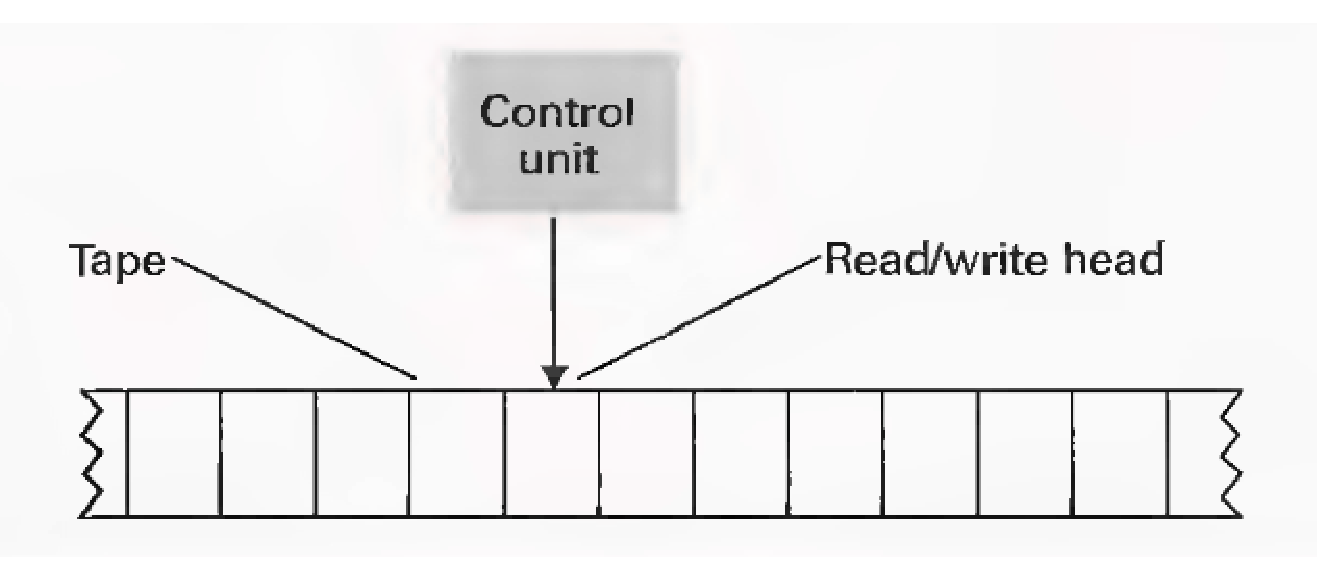
\includegraphics{ch7/fig112.pdf}}
  \caption{Các thành phần của một máy Turing}
\label{fig:fig112}
\end{figure}

Tại mỗi thời điểm tính toán, máy Turing ở một trạng thái nào đó và số trạng thái của máy
là hữu hạn. Một tính toán của máy Turing bắt đầu ở một trạng thái đặc biệt được gọi là
trạng thái bắt đầu và máy dừng khi đạt đến một trạng thái đặc biệt, gọi là trạng thái
dừng.


Một tính toán của máy Turing bao gồm một dãy các bước được thực hiện bởi đơn vị điều
khiển. Mỗi bước bao gồm việc quan sát ký hiệu ở ô hiện hành (ô này được nhìn bởi đầu
đọc/ghi) trên băng, viết một ký hiệu lên ô, có khả năng chuyển đầu đọc sang ô bên trái
hoặc bên phải, và sau đó thay đổi trạng thái. Hoạt động máy phải thực hiện được xác định
bởi một chương trình, nó dựa vào trạng thái của máy và nội dung của ô nhớ hiện thời trên
băng để chỉ ra đơn vị điều khiển phải làm gì .

Ta cùng xem xét một ví dụ về một máy Turing. Để tiện lợi, ta biểu diễn băng của máy như
một đường thẳng nằm ngang chia thành các ô. Trên mỗi ô này ta có thể ghi một ký hiệu thuộc
bảng chữ của máy. Ta chỉ ra vị trí hiện thời của đầu đọc/ghi bằng cách đặt một nhãn dưới ô
nhớ hiện thời. Bộ chữ máy trong ví dụ của ta bao gồm các ký hiệu $0,1$ và $*$. Băng của
máy có thể xuất hiện như sau:
\begin{center}
   \scalebox{0.45}{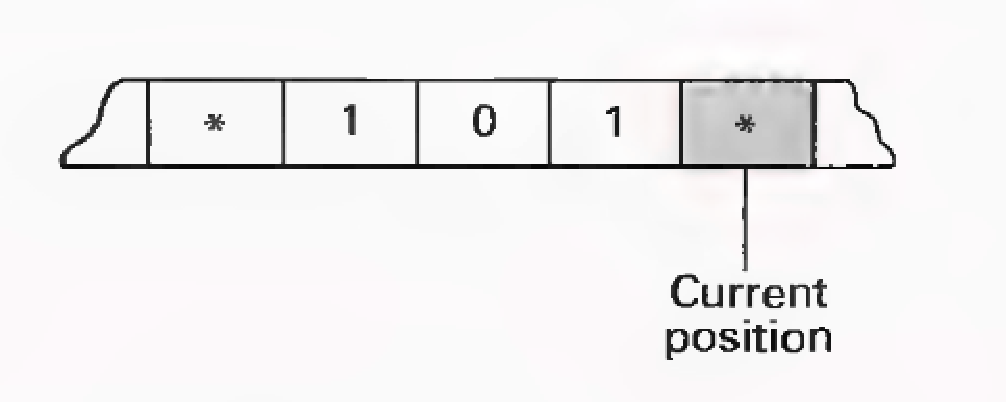
\includegraphics{ch7/turing1.pdf}}
\end{center}
%\end{wrapfigure}

Bằng cách diễn giải xâu ký hiệu trên băng như các biểu diễn nhị phân của các số nguyên
được ngăn cách bởi các dấu sao, ta thấy băng ở trên chứa giá trị $5$. Máy Turing của ta sẽ
được thiết kế để tăng giá trị trên băng lên $1$. Nói chính xác hơn, nó giả sử rằng vị trí
bắt đầu tại dấu sao bên phải của xâu gồm $0$ và $1$, và nó thực hiện biến đổi xâu thành
xâu biểu diễn số nguyên tiếp theo.

Các trạng thái của máy là \texttt{START}, \texttt{ADD}, \texttt{CARRY}, \texttt{OVERFLOW},
\texttt{RETURN}, và \texttt{HALT}. Các hoạt động tương ứng với mỗi trạng thái và nội dung
của ô hiện hành được mô tả theo bảng trong trong Hình~\ref{fig:fig113}.
 
Ta cùng chạy máy này trên băng biểu diễn giá trị $5$ trong hình trước. Máy bắt đầu ở trạng
thái \texttt{START} và ô nhớ hiện thời chứa $*$. Ta thực hiện theo chỉ dẫn ở bảng trên:
ghi lại giá trị $*$, chuyển đầu đọc/ghi sang trái một ô, và máy chuyển sang trạng thái
\texttt{ADD}. Máy bây giờ được mô tả như dưới đây:
\begin{center}
   \scalebox{0.45}{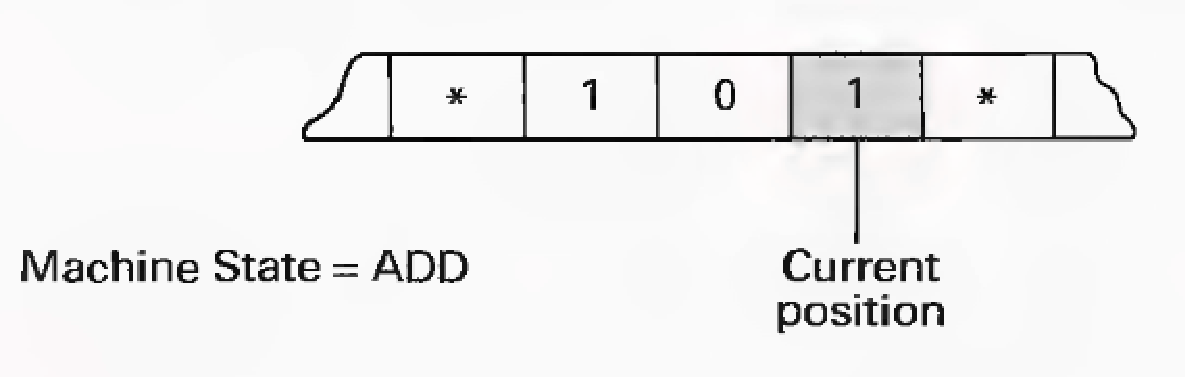
\includegraphics{ch7/turing2.pdf}}
\end{center}


Ta tiếp tục nhìn bảng trên để xem phải làm gì khi máy ở trạng thái \texttt{ADD} và ô hiện
tại chứa giá trị $0$. Bảng trên chỉ ra: thay thế $1$ ở ô nhớ hiện tại bởi $0$, chuyển đầu
đọc/ghi sang trái một ô, và máy chuyển sang trạng thái \texttt{CARRY}. Bây giờ hình trạng
của máy trở thành:
\begin{center}
   \scalebox{0.45}{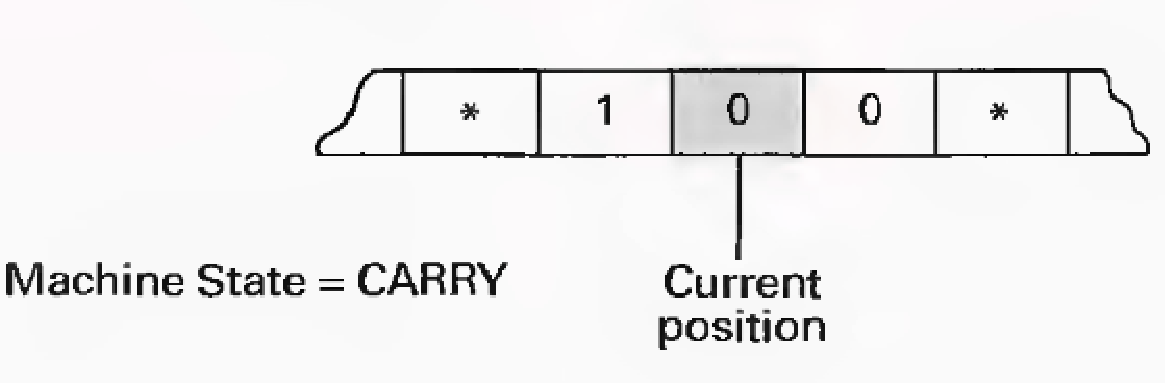
\includegraphics{ch7/turing3.pdf}}
\end{center}

Ta lại xem bảng trên để xem phải làm gì tiếp và thấy rằng khi máy ở trạng thái
\texttt{CARRY} với ô hiện hành chứa $0$, ta phải thay $0$ bằng $1$, chuyển đầu đọc/ghi
sang phải, và máy chuyển sang trạng thái \texttt{RETURN}. Bây giờ hình trạng của máy như
sau:
\begin{center}
   \scalebox{0.45}{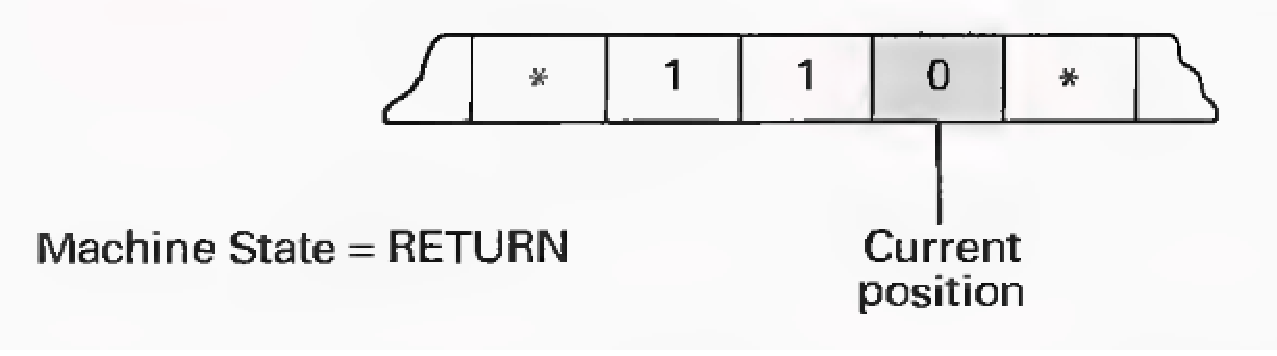
\includegraphics{ch7/turing4.pdf}}
\end{center}


Từ tình huống này, bảng trước chỉ ra ta phải thay $0$ ở ô hiện thời với giá trị $0$ khác,
chuyển đầu đọc/ghi sang phải, và máy vẫn ở trạng thái \texttt{RETURN}. Vậy máy ở trong
điều kiện sau đây:
\begin{center}
   \scalebox{0.45}{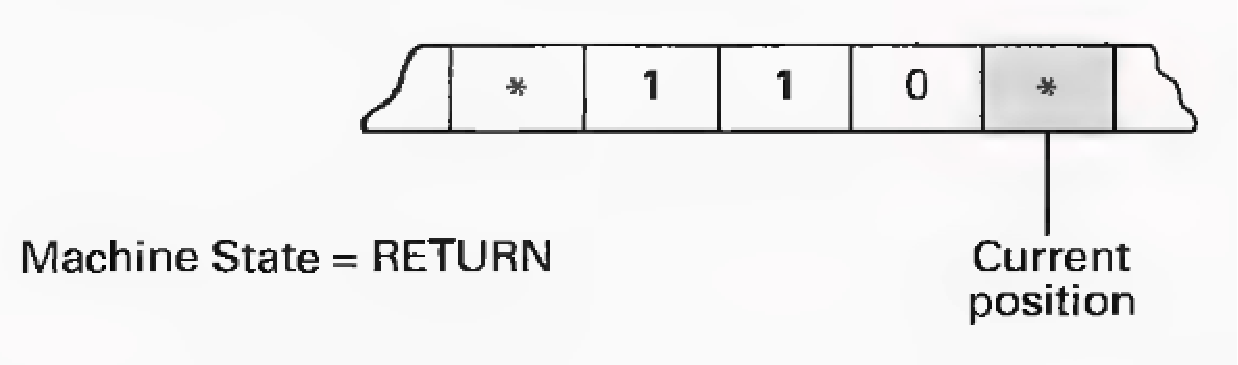
\includegraphics{ch7/turing5.pdf}}
\end{center}

Tại thời điểm này, ta thấy bảng trên chỉ ra rằng viết lại dấu sao trong ô hiện thời và máy
chuyển sang trạng thái \texttt{HALT}. Vậy máy dừng ở hình trạng sau đây (các ký hiệu trên
băng bây giờ biểu diễn giá trị $6$ đúng như ta mong đợi):
\begin{center}
   \scalebox{0.45}{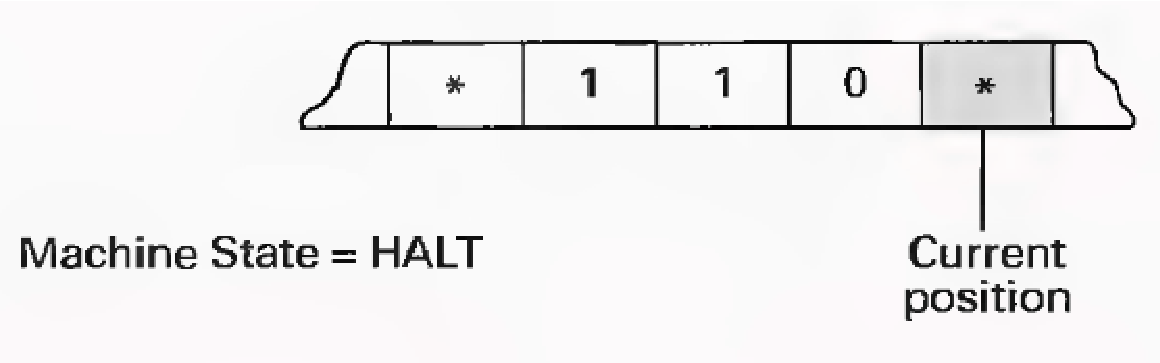
\includegraphics{ch7/turing6.pdf}}
\end{center}


\begin{figure}
  \label{fig:fig113}  
  \centering
  \begin{tabular}{ccccc} \hline
    \textbf{Trạng thái} & \textbf{Nội dung ô nhớ} & \textbf{Giá trị} & \textbf{Hướng di chuyển} & \textbf{Trạng thái} \\
    \textbf{hiện thời}  & \textbf{hiện thời}      & \textbf{cần ghi} &                          & \textbf{tiếp theo}  \\
    \hline
    \texttt{START}      & $*$                     & $*$              & sang Trái                & \texttt{ADD}        \\
    \texttt{ADD}        & $0$                     & $1$              & sang Phải                & \texttt{RETURN}     \\
    \texttt{ADD}        & $1$                     & $0$              & sang Trái                & \texttt{CARRY}      \\
    \texttt{ADD}        & $*$                     & $*$              & sang Phải                & \texttt{HALT}       \\
    \texttt{CARRY}      & $0$                     & $1$              & sang Phải                & \texttt{RETURN}     \\
    \texttt{CARRY}      & $1$                     & $0$              & sang Trái                & \texttt{CARRY}      \\
    \texttt{CARRY}      & $*$                     & $1$              & sang Trái                & \texttt{OVERFLOW}   \\
    \texttt{OVERFLOW}   & $*$                     & $*$              & sang Phải                & \texttt{RETURN}     \\
    \texttt{RETURN}     & $0$                     & $0$              & sang Phải                & \texttt{RETURN}     \\
    \texttt{RETURN}     & $1$                     & $1$              & sang Phải                & \texttt{RETURN}     \\
    \texttt{RETURN}     & $*$                     & $*$              & không chuyển             & \texttt{HALT}       \\
    \hline
  \end{tabular}
  \caption{Một máy Turing tăng giá trị}
\end{figure}

\subsection*{Luận đề Church-Turing}
Máy Turing trong phần trước được sử dụng để tính hàm tìm số liền sau, gắn mỗi giá trị đầu
vào là số nguyên không âm $n$ với giá trị đầu ra $n + 1$. Công việc của ta đơn thuần chỉ
là chuyển giá trị đầu vào thành dạng nhị phân và đặt lên băng của máy, để máy chạy cho tới
khi nó dừng, và sau đó đọc giá trị đầu ra trên băng. Một hàm có thể được tính bởi máy
Turing theo cách này được gọi là \textbf{tính được bằng máy Turing}.

Giả thiết của Turing là các hàm tính được bằng máy Turing cũng chính là các hàm tính
được. Nói cách khác, ông giả sử rằng khả năng tính toán của máy Turing chứa mọi hệ thống
thuật toán. Hay tương đương, mọi hàm tính được đều là hàm tính được bởi một máy Turing nào
đó. Giả thuyết này ngày nay được gọi là \textbf{luận đề Church-Turing}, để tưởng nhớ tới
các đóng góp của Alan~Turing và Alonzo~Church. Luận đề này không được chứng minh chặt chẽ
bằng toán học, tuy nhiên cho đến nay thực tiễn luôn chứng minh rằng luận đề đó là đúng đắn
và được chấp nhận rộng rãi. Có nghĩa rằng, hàm tính được và các hàm tính được bởi máy
Turing được xem xét là trùng nhau.

Điều đáng chú ý của giả thuyết này là nó cho ta nhận thức về khả năng và giới hạn của
máy. Chính xác hơn, nó thiết lập khả năng của các máy Turing như một chuẩn để các hệ thống
tính toán khác có thể so sánh. Nếu một hệ thống nào đó có khả năng tính toán mọi hàm có
thể tính bới máy Turing, thì nó được xem như có khả năng mạnh nhất mà mọi hệ thống tính
toán có thể.

\subsection*{Câu hỏi \& Bài tập}
\begin{enumerate}
\item Chạy máy Turing được mô tả trong mục này (Hình~\ref{fig:fig113}), nhưng với trạng
  thái khởi đầu sau đây:
\begin{center}
   \scalebox{0.45}{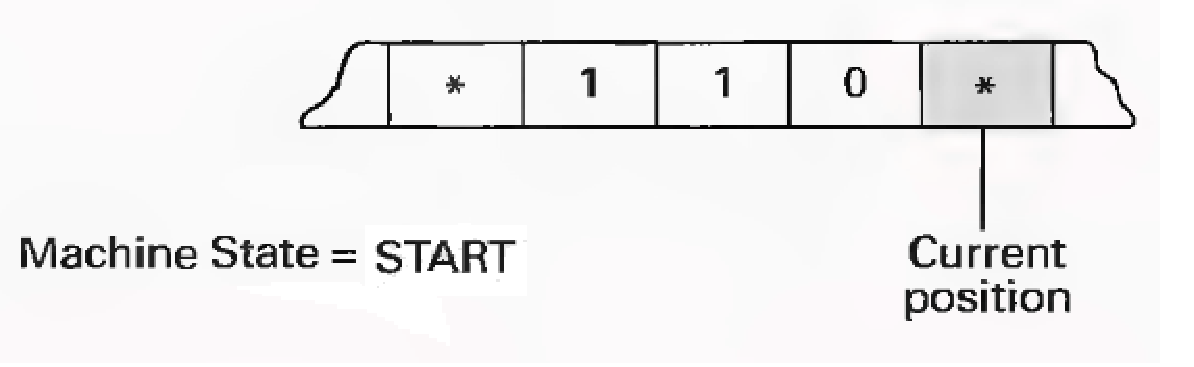
\includegraphics{ch7/turing7.pdf}}
\end{center}

\item Mô tả một máy Turing thay thế các xâu gồm các chữ $0$ và $1$ thành xâu chỉ gồm một
  chữ $0$.

\item Mô tả một máy Turing giảm giá trị trên băng đi một nếu giá trị đó lớn hơn không hoặc
  để nguyên nếu giá trị đó bằng không.

\item Chỉ ra một tình huống ngoài đời thường mà phải thực hiện tính toán. Tình huống này
  tương tự với một máy Turing như thế nào?

\item Mô tả một máy Turing dừng với một số đầu vào nhưng không bao giờ dừng với các đầu
  vào khác.
\end{enumerate}



%%% Local Variables: 
%%% mode: latex
%%% TeX-master: "../tindaicuong"
%%% End: 

\section{Các ngôn ngữ lập trình phổ dụng}
Trong Chương~\ref{ch6} ta đã nghiên cứu nhiều đặc điểm của ngôn ngữ lập trình bậc
cao. Trong mục này ta sẽ áp dụng kiến thức về tính toán để xác định những đặc điểm nào là
thực sự cần thiết. Ta sẽ thấy rằng hầu hết những đặc điểm của ngôn ngữ bậc cao ngày nay
thực ra chỉ giúp tiện lợi khi sử dụng hơn là đóng vai trò làm tăng khả năng cơ bản của
ngôn ngữ.

Cách tiếp cận của ta là mô tả một ngôn ngữ ra lệnh cho phép ta biểu diễn các chương trình
tính mọi hàm tính được bởi máy Turing (hay tương đương là mọi hàm tính được). Bởi vậy, nếu
một lập trình viên trong tương lai thấy một bài toán không thể giải được dùng ngôn ngữ
này, lý do sẽ không phải do hạn chế của ngôn ngữ mà là do không có thuật toán để giải
quyết bài toán đó. Một ngôn ngữ lập trình với tính chất này được gọi là \textbf{ngôn ngữ
  lập trình phổ dụng}.

Bạn sẽ ngạc nhiên khi thấy rằng một ngôn ngữ lập trình phổ dụng không nhất thiết phải phức
tạp. Thay vào đó, ngôn ngữ mà ta trình bày khá đơn giản. Ta sẽ gọi nó là Bare~Bones bởi vì
nó chỉ gồm tập tối thiểu các yêu cầu của một ngôn ngữ lập trình phổ dụng.

\subsection*{Ngôn ngữ Bare Bones}

Ta bắt đầu bằng việc xem xét các khai báo trong các ngôn ngữ lập trình. Các khai báo này
cho phép người lập trình suy nghĩ về các cấu trúc dữ liệu và kiểu dữ liệu (như mảng các
giá trị số hay xâu ký tự thuộc bảng chữ nào đó) dù máy chỉ đơn thuần thao tác với các bít
chứ không quan tâm đến các xâu biểu diễn gì. Trước khi đưa vào máy để thực hiện, một lệnh
ở mức cao liên quan đến các kiểu dữ liệu và cấu trúc phải được dịch thành các lệnh ở mức
máy để thao tác với các xâu bít để mô phỏng các hoạt động được yêu cầu.

Để thuận tiện, ta có thể diễn giải các xâu bít này như những biểu diễn nhị phân của các
giá trị nguyên không âm. Bởi vậy, không mất tổng quát mọi tính toán thực hiện bởi một máy
có thể được xem như các tính toán liên quan đến các số nguyên không âm. Và các ngôn ngữ
lập trình có thể được đơn giản hoá bằng cách yêu cầu người lập trình biểu diễn thuật toán
theo cách này (dù rằng điều này có thể gây khó khăn hơn trong lập trình).

Vì mục đích của ta là phát triển ngôn ngữ Bare~Bones đơn giản nhất có thể nên ta sẽ chọn
cách diễn giải này. Có nghĩa rằng, mọi biến trong Bare~Bones sẽ được xem xét như một dãy
bít, và được diễn giải như một số nguyên không âm theo ký hiệu nhị phân. Ví dụ, biến có
giá trị là xâu bít $10$ sẽ được gọi là chứa giá trị hai, và biến được gán bởi xâu bít
$101$ được gọi là chứa giá trị năm.

Theo cách này, mọi biến trong một chương trình Bare~Bones có cùng kiểu, nên ta không cần
khai báo xem tên biến và kiểu của nó là gì. Khi dùng Bare~Bones, lập trình viên có thể
dùng luôn biến mới khi cần, và hiểu rằng nó luôn tham chiếu tới một xâu bít diễn giải như
một giá trị nguyên không âm.

Tất nhiên, bộ dịch cho ngôn ngữ Bare Bone phải có khả năng phân biệt các tên biến với các
từ khác. Điều này được chỉ ra bởi cú pháp của Bare~Bones sao cho vai trò của mọi từ được
xác định bởi cú pháp duy nhất. Với mục đích này, ta quy định rằng tên biến phải bắt đầu
bởi một chữ trong bảng chữ tiếng Anh, và theo sau bởi một tổ hợp các chữ hoặc số (từ $0$
đến $9$). Vậy các xâu \texttt{XYZ}, \texttt{B747}, \texttt{abcdefghi}, và \texttt{X5Y} có
thể được sử dụng như tên biến, trong khi \texttt{2G5}, \texttt{\%o}, và \texttt{x.y} không
phải.

Ta cùng xem xét các lệnh trong Bare~Bones. Ngôn ngữ này có ba lệnh gán và một lệnh điều
khiển biểu diễn việc lặp. Ngôn ngữ này không có định dạng (free-format), bởi vậy mỗi lệnh
phải kết thúc bởi một dấu chấm phảy, điều này để dễ dàng dịch các lệnh riêng nhưng đặt
trên cùng một dòng. Tuy vậy, để dễ đọc ta thường đặt chỉ một lệnh trên một dòng.

Cả ba lệnh gán của ngôn ngữ Bare~Bones đều yêu cầu các nội dung của biến gán cũng chính là
biến yêu cầu được thay đổi trong lệnh. Lệnh đầu tiên cho phép ta gán giá trị không cho một
biến. Cú pháp của nó là
\begin{flushleft}
 \qquad \qquad \qquad \texttt{clear \textit{tên};}
\end{flushleft}
với \texttt{tên} có thể là mọi tên biến có thể.

Hai lệnh gán còn lại về cơ bản là ngược nhau
\begin{flushleft}
  \qquad\qquad\qquad\texttt{incr \textit{tên};}
\end{flushleft}
và
\begin{flushleft}
 \qquad\qquad\qquad \texttt{decr \textit{tên};}
\end{flushleft}
Một lần nữa, \texttt{\it tên} biểu diễn mọi tên biến. Lệnh trước làm tăng giá trị của biến
lên một và gán lại vào chính nó. Bởi vậy nếu biến \texttt{Y} đã có giá trị năm trước đó
thì lệnh
\begin{flushleft}
 \qquad\qquad\qquad \texttt{incr Y;}
\end{flushleft}
sau khi được thực hiện sẽ làm giá trị của \texttt{Y} tăng lên thành sáu.

Ngược lại, lệnh \texttt{decr} được dùng để làm giảm giá trị của biến đi một và gán lại cho
chính biến đó. Có một ngoại lệ là khi biến đã được gán bằng không thì lệnh không làm thay
đổi giá trị nữa. Bởi vậy, nếu giá trị của \texttt{Y} là năm thì sau khi lệnh
\begin{flushleft}
\qquad\qquad\qquad  \texttt{decr Y;}
\end{flushleft}
được thực hiện thì giá trị bốn sẽ được gán cho \texttt{Y}. Tuy nhiên, nếu giá trị của
\texttt{Y} đã bằng không thì giá trị này vẫn là không sau khi lệnh được thực hiện.

Bare~Bones chỉ cung cấp một cấu trúc điều khiển biểu diễn bởi cặp \texttt{while-end}. Dãy
lệnh sau
\begin{flushleft}
  \qquad \qquad\qquad \texttt{while \textit{tên} not 0 do;} \\
  \qquad\qquad\qquad\quad \texttt{.} \\
  \qquad\qquad\qquad\quad \texttt{.} \\
  \qquad\qquad\qquad\quad \texttt{.} \\
  \qquad\qquad\qquad\texttt{end;}
\end{flushleft}
(ở đó \texttt{tên} biểu diễn mọi tên biến có thể) sẽ thực hiện lặp lại một lệnh hoặc một
dãy lệnh nằm giữa cặp \texttt{while} và \texttt{end} cho đến khi giá trị của biến
\texttt{\it tên} bằng không. Chính xác hơn, nếu bắt gặp một cấu trúc \texttt{while-end}
khi đang thực hiện chương trình thì đầu tiên giá trị của biến được so sánh với không. Nếu
nó bằng không, cấu trúc này bị bỏ qua, và tiếp tục thực hiện tiếp lệnh ngay sau lệnh
\texttt{end}. Tuy vậy, nếu giá trị của biến khác không, dãy lệnh bên trong cấu trúc
\texttt{while-end} được thực hiện và điều khiển được trả lại vị trí của lệnh
\texttt{while}, và lúc này việc so sánh lại được thực hiện một lần nữa. Chú ý rằng khó
khăn của việc điều khiển lặp được đặt cho người lập trình, anh ta phải xác định rõ ràng
giá trị của biến nào bị thay đổi trong thân vòng lặp để tránh vòng lặp vô hạn. Ví dụ, dãy
lệnh
\begin{flushleft}
  \qquad \qquad\qquad \texttt{incr X;}\\
  \qquad \qquad\qquad \texttt{while \textit{X} not 0 do;} \\
  \qquad \qquad\qquad \quad \texttt{incr Z;} \\
  \qquad\qquad\qquad\texttt{end;}
\end{flushleft}
cho kết quả là một quá trình vô hạn vì khi lệnh \texttt{while} thực hiện, giá trị của
\texttt{X} không bao giờ bằng không, trong khi đó dãy
\begin{flushleft}
  \qquad \qquad\qquad \texttt{incr X;} \\
  \qquad \qquad\qquad \texttt{while \textit{X} not 0 do;} \\
  \qquad \qquad\qquad \quad \texttt{incr Z;} \\
  \qquad \qquad\qquad \quad \texttt{incr X;} \\
  \qquad\qquad\qquad\texttt{end;}
\end{flushleft}
cuối cùng cũng sẽ dừng và đặt giá trị ban đầu của \texttt{X} cho \texttt{Z}.

Để ý rằng các lệnh \texttt{while} và \texttt{end} phải xuất hiện theo cặp và lệnh
\texttt{while} phải xuất hiện trước. Tuy vậy, một lệnh \texttt{while-end} có thể xuất hiện
bên trong các lệnh lặp bằng cách đặt nó trong một cặp \texttt{while-end} khác. Trong các
trường hợp như thế này cặp \texttt{while} và \texttt{end} được hoàn thành bằng cách xem
xét toàn bộ chương trình để gắn mỗi lệnh \texttt{end} với lệnh \texttt{while} gần nó nhất
mà chưa được ghép cặp. Mặc dù không cần thiết về mặt cú pháp nhưng chúng ta thường sắp xếp
thụt vào để dễ đọc đối với các cấu trúc kiểu này.


Một ví dụ để kết thúc mục này là dãy lệnh trong Hình~\ref{fig:fig114}. Dãy lệnh này thực
hiện tính tích của các giá trị trong \texttt{X} và \texttt{Y} sau đó gán vào \texttt{Z},
mặt khác nó cũng ảnh hưởng đến giá trị ban đầu của \texttt{X}. (Cấu trúc
\texttt{while-end} được điều khiển bởi biến \texttt{W} nhằm lưu trữ giá trị gốc cho biến
\texttt{Y}.)

\begin{figure}[tbh]
  \begin{flushleft}
    \qquad \qquad\qquad  \texttt{clear Z;}\\
    \qquad \qquad\qquad \texttt{while X not 0 do;} \\
    \qquad \qquad\qquad \qquad \texttt{clear W;} \\
    \qquad \qquad\qquad \qquad \texttt{while Y not 0 do;} \\
    \qquad \qquad\qquad \qquad \qquad \texttt{incr Z;} \\
    \qquad \qquad\qquad \qquad \qquad \texttt{incr W;} \\
    \qquad \qquad\qquad \qquad \qquad \texttt{decr Y;} \\
    \qquad \qquad\qquad \qquad \texttt{end;} \\
    \qquad \qquad\qquad \qquad \texttt{while W not 0 do;} \\
    \qquad \qquad\qquad \qquad \qquad \texttt{incr Y;}\\
    \qquad \qquad\qquad \qquad \qquad \texttt{decr W;}\\
    \qquad \qquad\qquad \qquad \texttt{end;} \\
    \qquad \qquad\qquad \qquad \texttt{decr X;} \\
    \qquad\qquad\qquad\texttt{end;}
\end{flushleft}
  \caption{Một chương trình Bare Bone để tính \texttt{X*Y}}
  \label{fig:fig114}
\end{figure}

\subsection*{Lập trình Bare Bone}
Ta nhắc lại rằng mục đích của việc trình bày Bare~Bones là để thảo luận về khả năng về mặt
lý thuyết và thực tế của máy. Bare~Bones có thể rất khó khăn trong ứng dụng thực tế. Tuy
nhiên, như ta sẽ thấy ngay trong mục sau, nó lại cho ta mọi khả năng của một ngôn ngữ lập
trình phổ dụng. Bây giờ, ta sẽ xem xét xem làm thế nào mà Bare~Bones có thể được dùng để
biểu diễn một vài thao tác cơ bản.

Đầu tiên ta để ý rằng bằng cách tổ hợp các lệnh gán, ta có thể gán cho một biến một giá
trị tuỳ ý ( mọi số nguyên không âm). Ví dụ, dãy lệnh sau đây gán giá trị ba cho
biến~\texttt{X} bằng cách đầu tiên gán nó với giá trị không và sau đó tăng giá trị này lên
ba lần:
\begin{flushleft}
\qquad\qquad\qquad  \texttt{clear X;} \\
\qquad\qquad\qquad  \texttt{incr X;} \\
\qquad\qquad\qquad  \texttt{incr X;} \\
\qquad\qquad\qquad  \texttt{incr X;}
\end{flushleft}

Một thao tác phổ biến khác là sao chép dữ liệu từ một vị trí tới vị trí khác. Nói theo
cách của ngôn ngữ Bare~Bones, ta cần gán giá trị một biến bằng một biến khác. Điều này có
thể thực hiện bằng cách xoá biến cần gán và sau đó lặp lại việc tăng nó lên một số lần
thích hợp. Thực ra ta thấy rằng dãy lệnh
\begin{flushleft}
\qquad\qquad\qquad  \texttt{clear Z;} \\
\qquad\qquad\qquad  \texttt{while  X not 0 do;} \\
\qquad\qquad\qquad  \qquad \texttt{incr Z;} \\
\qquad\qquad\qquad  \qquad \texttt{decr X;} \\
\qquad\qquad\qquad  \texttt{incr X;}
\end{flushleft}
chuyển giá trị được gắn với \texttt{X} cho \texttt{Z}. Tuy vậy, dãy lệnh này lại phá huỷ
giá trị của \texttt{X}. Để tránh điều này, ta dùng một biến tạm để chuyển dữ liệu ban đầu
vào biến này. Sau đó ta dùng biến tạm này làm dữ liệu nguồn để lưu trữ lại giá trị của biến
gốc, đồng thời gán giá trị có biến cần gán bằng biến gốc. Theo cách này, việc chuyển dữ
liệu từ biến \texttt{Today} thành \texttt{Yesterday} có thể được thực hiện dùng dãy lệnh
như trong Hình~\ref{fig:fig115}.


Ta chọn cú pháp
\begin{flushleft}
\qquad\qquad\qquad  \texttt{copy \textit{tên1} to \textit{tên2};}
\end{flushleft}
(với \texttt{tên1} và \texttt{tên2} biển diễn các tên biến) như kí hiệu viết tắt cho một
cấu trúc lệnh có dạng như Hình~\ref{fig:fig115}. Bởi vậy, mặc dù Bare~Bones bản thân nó
không có lệnh \texttt{copy}, ta thường viết chương trình có lệnh này, và ta ngầm hiểu rằng
ta đã chuyển một cách không hình thức thành các chương trình Bare~Bones thực sự bằng cách
thay thế lệnh \texttt{copy} bằng các cấu trúc \texttt{while-end} thích hợp (với các biến
tạm có tên không xung đột với tên đã được sử dụng ở nơi khác trong chương trình.)

\begin{figure}[tbh]
  \begin{flushleft}
    \qquad \qquad\qquad  \texttt{clear Aux;}\\
    \qquad \qquad\qquad  \texttt{clear Tomorrow;}\\
    \qquad \qquad\qquad \texttt{while Today not 0 do;} \\
    \qquad \qquad\qquad \qquad \texttt{incr  Aux;} \\
    \qquad \qquad\qquad \qquad \texttt{decr Today;} \\
    \qquad \qquad\qquad \texttt{end;} \\

    \qquad\qquad \qquad \texttt{while Aux not 0 do;} \\
    \qquad\qquad \qquad \qquad \texttt{incr Today;} \\
    \qquad\qquad \qquad \qquad \texttt{incr Tomorrow;} \\
    \qquad\qquad \qquad \qquad \texttt{decr Aux;} \\
    \qquad\qquad \qquad \texttt{end;}
  \end{flushleft}
  \caption{Cài đặt hàm `` sao chép \texttt{Today} thành
    \texttt{Tomorrow}''}
  \label{fig:fig115}  
\end{figure}  

\subsection*{Tính phổ dụng của Bare Bones}
Bây giờ ta sẽ áp dụng luận đề Church-Turing để khẳng định rằng Bare~Bones là một ngôn ngữ
lập trình phổ dụng. Đầu tiên ta nhận thấy rằng mọi chương trình được viết trong Bare~Bones
có thể được nhìn như một việc tính toán hàm. Các hàm với đầu vào là các giá trị được gán
cho các biến trước khi thực hiện chương trình, và đầu ra của hàm là giá trị của các biến
khi chương trình kết thúc. Để tính hàm, ta đơn thuần chỉ chạy chương trình, bắt đầu
với việc khởi tạo giá trị cho các biến, và quan sát giá trị của các biến khi chương trình
kết thúc.

Dưới các điều kiện này, chương trình
\begin{flushleft}
\qquad\qquad\qquad  \texttt{incr X;}
\end{flushleft}
tính toán cùng một hàm (hàm tính số liền sau) được tính bởi máy Turing trong ví dụ trong
Mục~\ref{sec:112}. Thật vậy, nó tăng giá trị gắn với biến \texttt{X} lên một. Tương tự,
nếu chúng ta diễn giải các biến \texttt{X} và \texttt{Y} như các đầu vào và biến
\texttt{Z} như đầu ra thì chương trình
\begin{flushleft}
  \qquad \qquad\qquad  \texttt{copy Y to Z;}\\
  \qquad \qquad\qquad \texttt{while X not 0 do;} \\
  \qquad \qquad\qquad \qquad \texttt{incr  Z;} \\
  \qquad \qquad\qquad \qquad \texttt{decr X;} \\
  \qquad \qquad\qquad \texttt{end;} \\
\end{flushleft}
trực tiếp tính toán hàm cộng.

Các nhà nghiên cứu đã chứng minh rằng ngôn ngữ lập trình Bare~Bones có thể được sử dụng để
biểu diễn các thuật toán để tính mọi hàm tính được bởi máy Turing. Kết hợp với luận đề
Church-Turing nó chỉ ra rằng mọi hàm đều có thể được tính toán bởi một chương trình viết
bằng Bare~Bones. Bởi vậy Bare~Bones là một ngôn ngữ lập trình phổ dụng theo nghĩa rằng,
nếu có một thuật toán để giải quyết bài toán, thì bài toán đó có thể được giải bởi một
chương trình Bare~Bones nào đó. Nói tóm lại, Bare~Bones về mặt lý thuyết có thể dùng như
một ngôn ngữ lập trình đa năng.

Ta nói \textit{về mặt lý thuyết} vì một ngôn ngữ kiểu như thế này chắc chắn không tiện lợi
như các ngôn ngữ bậc cao đã được giới thiệu trong Chương~\ref{}. Tuy vậy, mỗi ngôn ngữ về
cơ bản đều chứa các đặc điểm của Bare~Bones như phần cơ bản nhất. Và phần cơ bản này đảm
bảo tính phổ dụng cho các ngôn ngữ bậc cao này; còn các đặc điểm thêm vào của ngôn ngữ chỉ
giúp làm cho nó thêm tiện lợi.

Mặc dù không thực tế trong môi trường lập trình ứng dụng, các ngôn ngữ kiểu Bare~Bones lại
hay được dùng trong nghiên cứu lý thuyết khoa học máy tính. Ví dụ, trong phụ lục~\ref{} ta
dùng Bare~Bones như một công cụ để giải quyết câu hỏi về tính tương đương của cấu trúc lặp
và cấu trúc đệ quy nảy sinh trong Chương~\ref{}. Nhờ công cụ này, nghi ngờ của ta về tính
tương đương của hai cấu trúc này đã được chứng minh.

\subsection*{Câu hỏi \& Bài tập}
\begin{enumerate}
\item Chỉ ra rằng lệnh \texttt{invert X;} (để chuyển các giá trị của \texttt{X} thành
  không nếu nó được khởi tạo khác không và thành một nếu nếu giá trị khởi tạo bằng không)
  có thể được mô phỏng bởi một đoạn chương trình Bare~Bones.

\item Chỉ ra rằng ngôn ngữ đơn giản Bare~Bones cũng chưa phải là tối thiểu bằng cách chứng
  minh rằng lệnh \texttt{clear} có thể được thay thế bằng tổ hợp của các lệnh khác trong
  ngôn ngữ.

\item Chỉ ra rằng cấu trúc \texttt{if-then-else} có thể mô phỏng dùng Bare~Bones. Có nghĩa
  rằng, bạn hãy viết một dãy lệnh trong Bare~Bones mô phỏng lệnh
  \begin{flushleft}
    \qquad \qquad  \texttt{if X not 0 then S1 else S2;}
  \end{flushleft}
  với \texttt{S1} và \texttt{S2} là một dãy lệnh bất kỳ.

\item Chỉ ra rằng mỗi lệnh Bare~Bones có thể biểu diễn theo ngôn ngữ máy ở Phụ
  lục~\ref{phuluc1} (Bởi vậy Bare~Bones có thể được sử dụng như một ngôn ngữ lập trình cho
  một máy kiểu này.)

\item Làm thế nào để có thể tính toán các số nguyên âm với Bare~Bones?

\item Mô tả hàm được tính bởi chương trình Bare~Bones sau đây, giả sử rằng đầu vào của hàm
  được biểu diễn bởi \texttt{X} và đầu ra bởi \texttt{Z}:
  \begin{flushleft}
    \qquad \qquad  \texttt{clear Z;}\\
    \qquad \qquad \texttt{while X not 0 do;} \\
    \qquad \qquad \qquad \texttt{incr  Z;} \\
    \qquad \qquad \qquad \texttt{incr  Z;} \\
    \qquad \qquad \qquad \texttt{decr  X;} \\
    \qquad \qquad \texttt{end;} 
  \end{flushleft}
\end{enumerate}

 
%%% Local Variables: 
%%% mode: latex
%%% TeX-master: "../tindaicuong"
%%% End: 

\section{Hàm không tính được}
\label{sec:114}
Bây giờ ta sẽ xác định một hàm không tính được bởi máy Turing, và theo luận đề
Church-Turing, người ta tin rằng nó không tính được theo nghĩa tổng quát. Vậy thì, việc
tính hàm này vượt ra ngoài khả năng của máy tính.

\subsection*{Bài toán dừng}

Hàm không tính được ta tìm thấy liên quan đến một bài toán, gọi là \textbf{bài toán
  dừng}. Nói một cách không hình thức, bài toán này tìm cách dự đoán xem một chương trình
sẽ kết thúc (hoặc dừng) hay không nếu nó bắt đầu ở một số điều kiện nào đó. Ví dụ, ta xem
xét chương trình Bare~Bones đơn giản sau đây
\begin{flushleft}
  \qquad \qquad\qquad \texttt{while X not 0 do;} \\
  \qquad \qquad\qquad \quad \texttt{incr X;} \\
  \qquad\qquad\qquad\texttt{end;}
\end{flushleft}
Nếu ta thực hiện chương trình này với giá trị khởi đầu của \texttt{X} bằng không, vòng lặp
sẽ không được thực hiện và chương trình sẽ kết thúc nhanh chóng. Tuy nhiên, nếu ta thực
hiện chương trình với các giá trị \texttt{X} nguyên dương, vòng lặp sẽ thực hiện mãi mãi,
và dẫn đến một quá trình không kết thúc.

Trong trường hợp này, ta dễ dàng kết luận rằng việc thực hiện chương trình sẽ dừng khi và
chỉ khi chương trình bắt đầu với giá trị \texttt{X} được khởi tạo bằng không. Tuy nhiên,
nếu xem xét các ví dụ phức tạp hơn, nhiệm vụ dự đoán hành vi của chương trình trở nên vô
cùng phức tạp. Và thực ra, như ta sẽ thấy, trong một vài trường hợp nhiệm vụ này là không
thể. Trước khi làm điều này, ta cần định nghĩa chính xác một vài thuật ngữ.

Ví dụ trước cho ta thấy rằng việc một chương trình có thể dừng hay không cũng phụ thuộc
vào việc khởi tạo các biến. Bởi vậy, nếu ta hy vọng có thể dự đoán khi nào chương trình sẽ
dừng, thì ta phải xem xét một cách cẩn thận giá trị khởi đầu của các biến trong chương
trình. Cách ta sẽ làm để chọn giá trị cho các biến có thể sẽ làm cho bạn cảm thấy hơi lạ
lúc đầu, nhưng bạn đừng quá lo lắng, mọi thứ sẽ dần dần được làm rõ. Mục đích của ta là
phát triển một kỹ thuật được gọi là \textbf{tự tham chiếu}--ý tưởng là tham chiếu một đối
tượng đến chính bản thân nó. Thủ thuật này đã dẫn đến nhiều kết quả đáng kinh ngạc trong
toán học, bắt đầu từ những câu đơn giản gây thắc mắc như ``Khẳng định này là sai'' tới
những nghịch lý như ``Có phải tập hợp tất cả các tập hợp có chứa chính nó?''. Ta cũng sẽ
dùng kỹ thuật này trong chứng minh của ta. Cụ thể, ta sẽ xây dựng một dãy các lập luận
kiểu như ``Nếu nó thực hiện, vậy nó không thực hiện; nhưng, nếu nó không thực hiện, vậy nó
thực hiện.''

Trong trường hợp của ta, tự tham chiếu sẽ được thực hiện bằng cách gán các biến trong
chương trình giá trị khởi đầu biểu diễn chính bản thân chương trình. Trước hết, ta để ý
rằng mỗi chương trình Bare~Bones có thể được mã hoá như một dãy bít với mỗi chữ trong
chương trình được mã bởi một byte ASCII, bởi vậy nó có thể được diễn giải như là biểu diễn
nhị phân của một số nguyên không âm (khá lớn). Đây chính là giá trị nguyên mà ta sẽ gán
cho các biến lúc khởi tạo chương trình.
 
Ta cùng xem xét một chương trình đơn giản 

\bigskip

\bigskip

\begin{flushleft}
  \qquad \qquad\qquad \texttt{while X not 0 do;} \\
  \qquad \qquad\qquad \quad \texttt{incr X;} \\
  \qquad\qquad\qquad\texttt{end;}
\end{flushleft}
Ta muốn biết chuyện gì xảy ra nếu ta bắt đầu chương trình này với \texttt{X} được gán cho
một giá trị nguyên biểu diễn chính bản thân chương trình (Hình~\ref{fig:fig116}). Trong
trường hợp này, ta nhanh chóng có câu trả lời. Do \texttt{X} có giá trị khác không, nên
chương trình sẽ rơi vào một vòng lặp vô hạn. Tuy vậy, nếu ta thử nghiệm tương tự với
chương trình
\begin{flushleft}
  \qquad \qquad\qquad \texttt{clear X;}\\
  \qquad \qquad\qquad \texttt{while X not 0 do;} \\
  \qquad \qquad\qquad \quad \texttt{incr X;} \\
  \qquad\qquad\qquad\texttt{end;}
\end{flushleft}
chương trình này luôn dừng vì biến \texttt{X} nhận giá trị bằng không trước cấu trúc
\texttt{while-end} mà không cần biết giá trị khởi đầu của \texttt{X} là gì.
\begin{figure}[tbh]
  \centering 
  \scalebox{0.5}{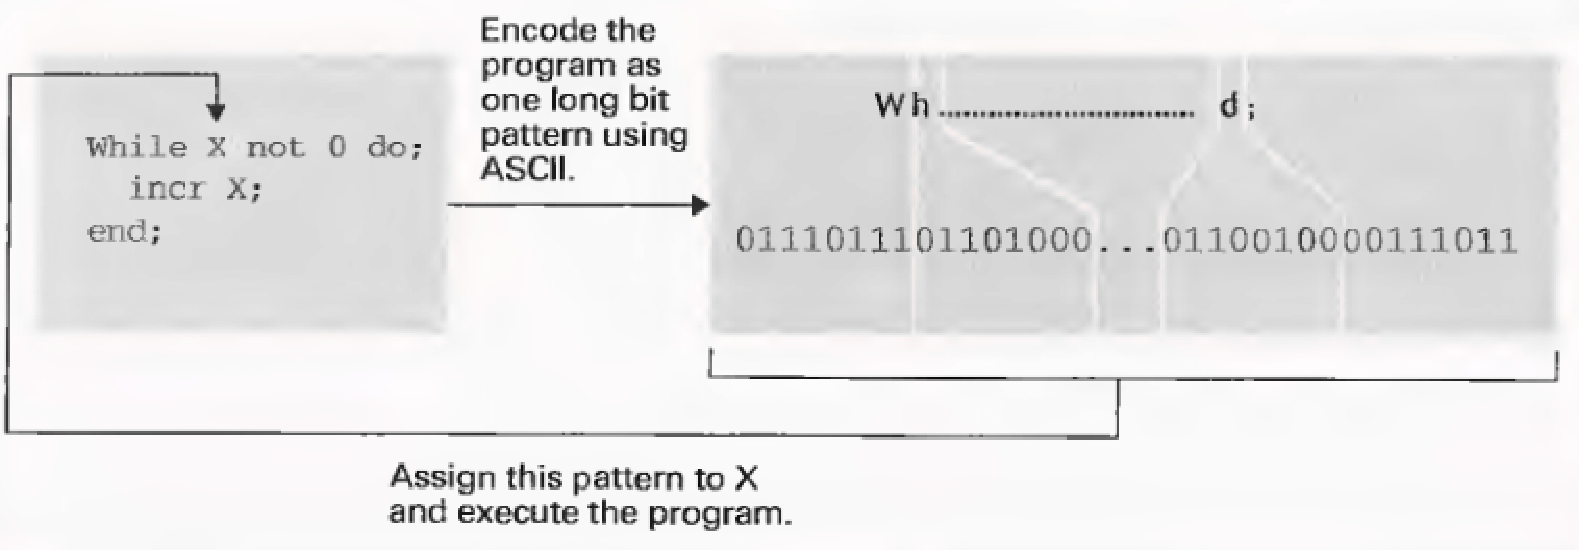
\includegraphics{ch7/fig116.pdf}}
  \caption{Kiểm tra một chương trình xem có tự kết thúc}
\label{fig:fig116}  
\end{figure}

Các ví dụ trên dẫn ta đến khái niệm \textbf{tự kết thúc} (seft-terminating). Một chương
trình Bare~Bones được gọi là tự kết thúc nếu ta khởi tạo các biến trong chương trình trước
khi thực hiện bằng chính mã hoá của chương trình thì việc thực hiện chương trình phải dẫn
đến một quá trình kết thúc. Hay nói nôm na, một chương trình gọi là tự kết thúc nếu ta
thực hiện nó với đầu vào là chính nó sẽ dừng sau một khoảng thời gian thực hiện. Đây chính
là khái niệm tự tham chiếu mà ta sẽ sử dụng trong chứng minh.

Để ý rằng một chương trình tự kết thúc có thể không làm đúng mục đích mà người viết mong
muốn. Ta có tính chất rằng một chương trình Bare~Bones phải hoặc tồn tại hoặc không tồn
tại. Và một chương trình Bare~Bones hoặc tự kết thúc hoặc không tự kết thúc.

Bây giờ ta mô tả bài toán dừng một cách chính xác. Đây là bài toán xác định xem một chương
trình Bare~Bones có tự kết thúc hay không. Ta sẽ thấy rằng không có thuật toán để trả lời
câu hỏi này trong trường hợp tổng quát. Có nghĩa rằng, không có thuật toán để khi đưa vào
một chương trình Bare~Bones, ta nhận được câu trả lời ``yes'' hoặc ``no'', tương ứng chỉ
chương trình có dừng hay không. Do đó lời giải của bài toán này vượt ra ngoài khả năng của
máy tính.

Có điều gì đó mâu thuẫn khi ta chỉ ra các bài toán ở ví dụ trước là giải được, mặt khác
lại khẳng định rằng bài toán dừng là không giải được. Ta sẽ giải thích điều này. Quan sát
ta dùng trong ví dụ trước chỉ là một trường hợp cụ thể và không thể áp dụng cho mọi tình
huống. Bài toán dừng yêu cầu chỉ ra một thuật toán tổng quát để có thể áp dụng với mọi
chương trình Bare~Bones. Khả năng chỉ ra trong một chương trình cụ thể có tự kết thúc hay
không sẽ không suy ra sự tồn tại một thuật toán tổng quát cho mọi trường hợp được. Nói tóm
lại, ta có thể xây dựng một máy giải một bài toán dừng với một đầu vào cụ thể, nhưng không
thể xây dựng một máy giải bài toán dừng với mọi đầu vào có thể.

\subsection*{Tính không giải được của bài toán dừng}

Bây giờ ta muốn chứng minh rằng việc giải bài toán dừng vượt ra ngoài khả năng của
máy. Cách tiếp cận của ta là chỉ ra việc giải bài toán cần đến một thuật toán để tính một
hàm không tính được. Đầu vào của hàm liên quan đến việc mã hoá chính phiên bản của chương
trình Bare Bones; đầu ra của nó giới hạn chỉ là giá trị $0$ hoặc $1$.  Nói chính xác hơn,
ta định nghĩa hàm thoả mãn: nếu đầu vào biểu diễn một chương trình tự kết thúc thì đầu ra
sẽ cho giá trị $1$, ngược lại đầu ra sẽ cho giá trị $0$. Để thuận tiện ta gọi hàm này là
\textit{hàm dừng}.


Nhiệm vụ của ta là chứng minh rằng hàm dừng là không tính được. Cách tiếp cận là dùng kỹ
thuật ``chứng minh phản chứng''. Nói ngắn gọn, ta chứng minh khẳng định là sai bằng cách
chỉ ra rằng nó không thể đúng. Ta sẽ chỉ ra rằng khẳng định ``hàm dừng là tính được'' là
không thể đúng. Các lập luận ta dùng để chứng minh điều này được tóm tắt trong
Hình~\ref{fig:fig117}.


Nếu hàm dừng là tính được, vậy (do Bare Bones là ngôn ngữ lập trình phổ dụng) phải có một
chương trình Bare~Bones tính nó. Nói một cách khác, có một chương trình Bare~Bones kết
thúc với đầu ra là $1$ nếu đầu vào của nó là phiên bản được mã hoá của một chương trình tự
kết thúc, ngược lại nó kết thúc với đầu ra là $0$.

Để sử dụng chương trình này ta không cần xác định biến đầu là gì vào mà đơn thuần chỉ khởi
tạo mọi biến của chương trình bằng biểu diễn được mã hoá của chương trình cần kiểm tra. Ta
có điều này bởi vì các biến không phải biến đầu vào vốn đã là các biến mà giá trị khởi tạo
của nó không ảnh hưởng đến đầu ra cuối cùng của chương trình. Ta kết luận rằng nếu hàm
dừng là có thể tính được, vậy thì có một chương trình Bare~Bones kết thúc với đầu ra bằng
$1$ nếu mọi biến của nó được khởi tạo bằng phiên bản được mã hoá của một chương trình tự
kết thúc, và kết thúc với đầu ra bằng $0$ trong trường hợp ngược lại.

Giả sử biến đầu ra của chương trình được đặt tên là \texttt{X} (nếu không ta có thể đổi
tên biến), ta thay đổi chương trình bằng cách thêm các lệnh
\begin{flushleft}
  \qquad \qquad\qquad \texttt{while X not 0 do;} \\
  \qquad\qquad\qquad\texttt{end;}
\end{flushleft}
vào cuối chương trình, và ta được một chương trình mới. Chương trình mới này phải hoặc là
tự kết thúc hoặc không. Tuy vậy, ta sẽ thấy rằng cả hai trường hợp đều không phải.

Đặc biệt, nếu chương trình mới này đã là tự kết thúc và ta đã chạy nó với các biến được
khởi tạo là biểu diễn được mã hoá của bản thân chương trình, vậy khi đó việc thực hiện của
nó tới lệnh \texttt{while} ta thêm vào, biến \texttt{X} phải chứa giá trị $1$. (Từ điểm
này ta thấy chương trình mới đồng nhất với chương trình ban đầu có đầu ra là $1$ nếu đầu
vào biểu diễn chương trình tự kết thúc.) Lúc này, việc thực hiện bài toán bị rơi vào vòng
lặp vô hạn vì không có lệnh nào giảm \texttt{X} trong vòng lặp. Nhưng điều này mâu thuẫn
vì giả sử của ta là chương trình mới này là tự kết thúc. Vậy ta kết luận rằng chương trình
này phải không tự kết thúc.

Tuy nhiên, nếu chương trình này đã không tự kết thúc và ta thực hiện nó với các biến được
khởi tạo là biểu diễn được mã hoá của chính chương trình đó, nó có thể dẫn tới vòng lặp
\texttt{while} với giá trị \texttt{X} được gán giá trị $0$. (Ta có điều này bởi vì khẳng
định trước lệnh \texttt{while} tạo thành chương trình gốc, và chương trình này có đầu ra
$0$ với đầu vào biểu diễn một chương trình không tự kết thúc.) Trong trường hợp này, cấu
trúc \texttt{while-end} không được thực hiện và chương trình phải dừng. Nhưng đây là tính
chất của chương trình tự kết thúc, vậy ta kết luận rằng chương trình mới này là tự kết
thúc, điều này mâu thuẫn với kết luận trước đó rằng đây là chương trình không tự kết thúc.

Tóm lại, ta thấy mâu thuẫn bởi vì một mặt ta có một chương trình phải hoặc tự kết thúc
hoặc không, mặt khác ta lại gặp tình huống cả hai đều sai. Vậy, giả sử của ta về ``hàm
dừng là tính được'' là sai.

Vậy ta đi đến kết luận rằng hàm dừng là không tính được, và do lời giải của bài toán dừng
liên quan đến tính toán hàm này, nên ta kết luận rằng việc giải bài toán dừng vượt ra
ngoài khả năng của mọi hệ thống thuật toán. Các bài toán kiểu này gọi là \textbf{bài toán
  không giải được}.



Cuối cùng, ta sẽ liên hệ những thảo luận vừa rồi với ý tưởng trong Chương~\ref{}. Ở đó,
câu hỏi chính là phải chăng khả năng của máy tính toán nằm trong khả năng cần thiết cho
chính bản thân trí thông minh. Nhắc lại rằng máy có chỉ có khả năng giải quyết vấn đề nếu
có lời giải thuật toán. Vậy thì câu hỏi này là liệu chăng nhận thức của con người tiến bộ
hơn so với việc thực hiện quá trình thuật toán. Nếu không, vậy thì giới hạn của ta đề cập
ở đây cũng chính là giới hạn của con người. Không cần phải nói ta cũng thấy đây là một vấn
đề gây tranh cãi và đôi khi là vấn đề nhạy cảm. Nếu, ví dụ, nhận thức của con người không
hơn các máy có thể lập trình, vậy thì ta có thể kết luận rằng khả năng của con người không
phải là vô hạn như ta vẫn nghĩ.



\subsection*{Câu hỏi \& Bài tập}
 
\begin{enumerate}
\item Chương trình Bare~Bones sau đây có tự kết thúc không? Hãy giải thích câu trả lời của
  bạn.
  \begin{flushleft}
    \qquad\qquad \texttt{incr X;} \\
    \qquad\qquad\texttt{decr Y;}
  \end{flushleft}

\item Chương trình Bare~Bones sau đây có tự kết thúc? Hãy giải thích câu trả lời của bạn.

  \begin{flushleft}
    \qquad \qquad \texttt{copy X to Y;} \\
    \qquad \qquad \texttt{incr Y;} \\
    \qquad\qquad\texttt{incr Y;} \\
    \qquad\qquad\texttt{while X not 0 do;} \\
    \qquad\qquad \qquad\texttt{decr X;} \\
    \qquad\qquad \qquad\texttt{decr X;} \\
    \qquad\qquad \qquad\texttt{decr Y;} \\
    \qquad\qquad \qquad\texttt{decr Y;} \\
    \qquad\qquad\texttt{end;} \\
    \qquad\qquad\texttt{decr Y;} \\
    \qquad\qquad\texttt{while Y not 0 do;} \\
    \qquad\qquad\texttt{end;}
  \end{flushleft} 


\item Có gì sai trong kịch bản sau đây?
  \begin{quote}
    Trong nhiều cộng đồng, mọi người sở hữu ngôi nhà của anh hay chị ta. Người thợ sơn
    nhà của cộng đồng yêu cầu sơn mọi ngôi nhà và chỉ những ngôi nhà này là không
    được sơn bởi chủ của chúng.
  \end{quote}
  (\textit{Gợi ý:} Ai sơn ngôi nhà của người thợ sơn?)
\end{enumerate}

\begin{figure}
  \centering 
  \scalebox{0.6}{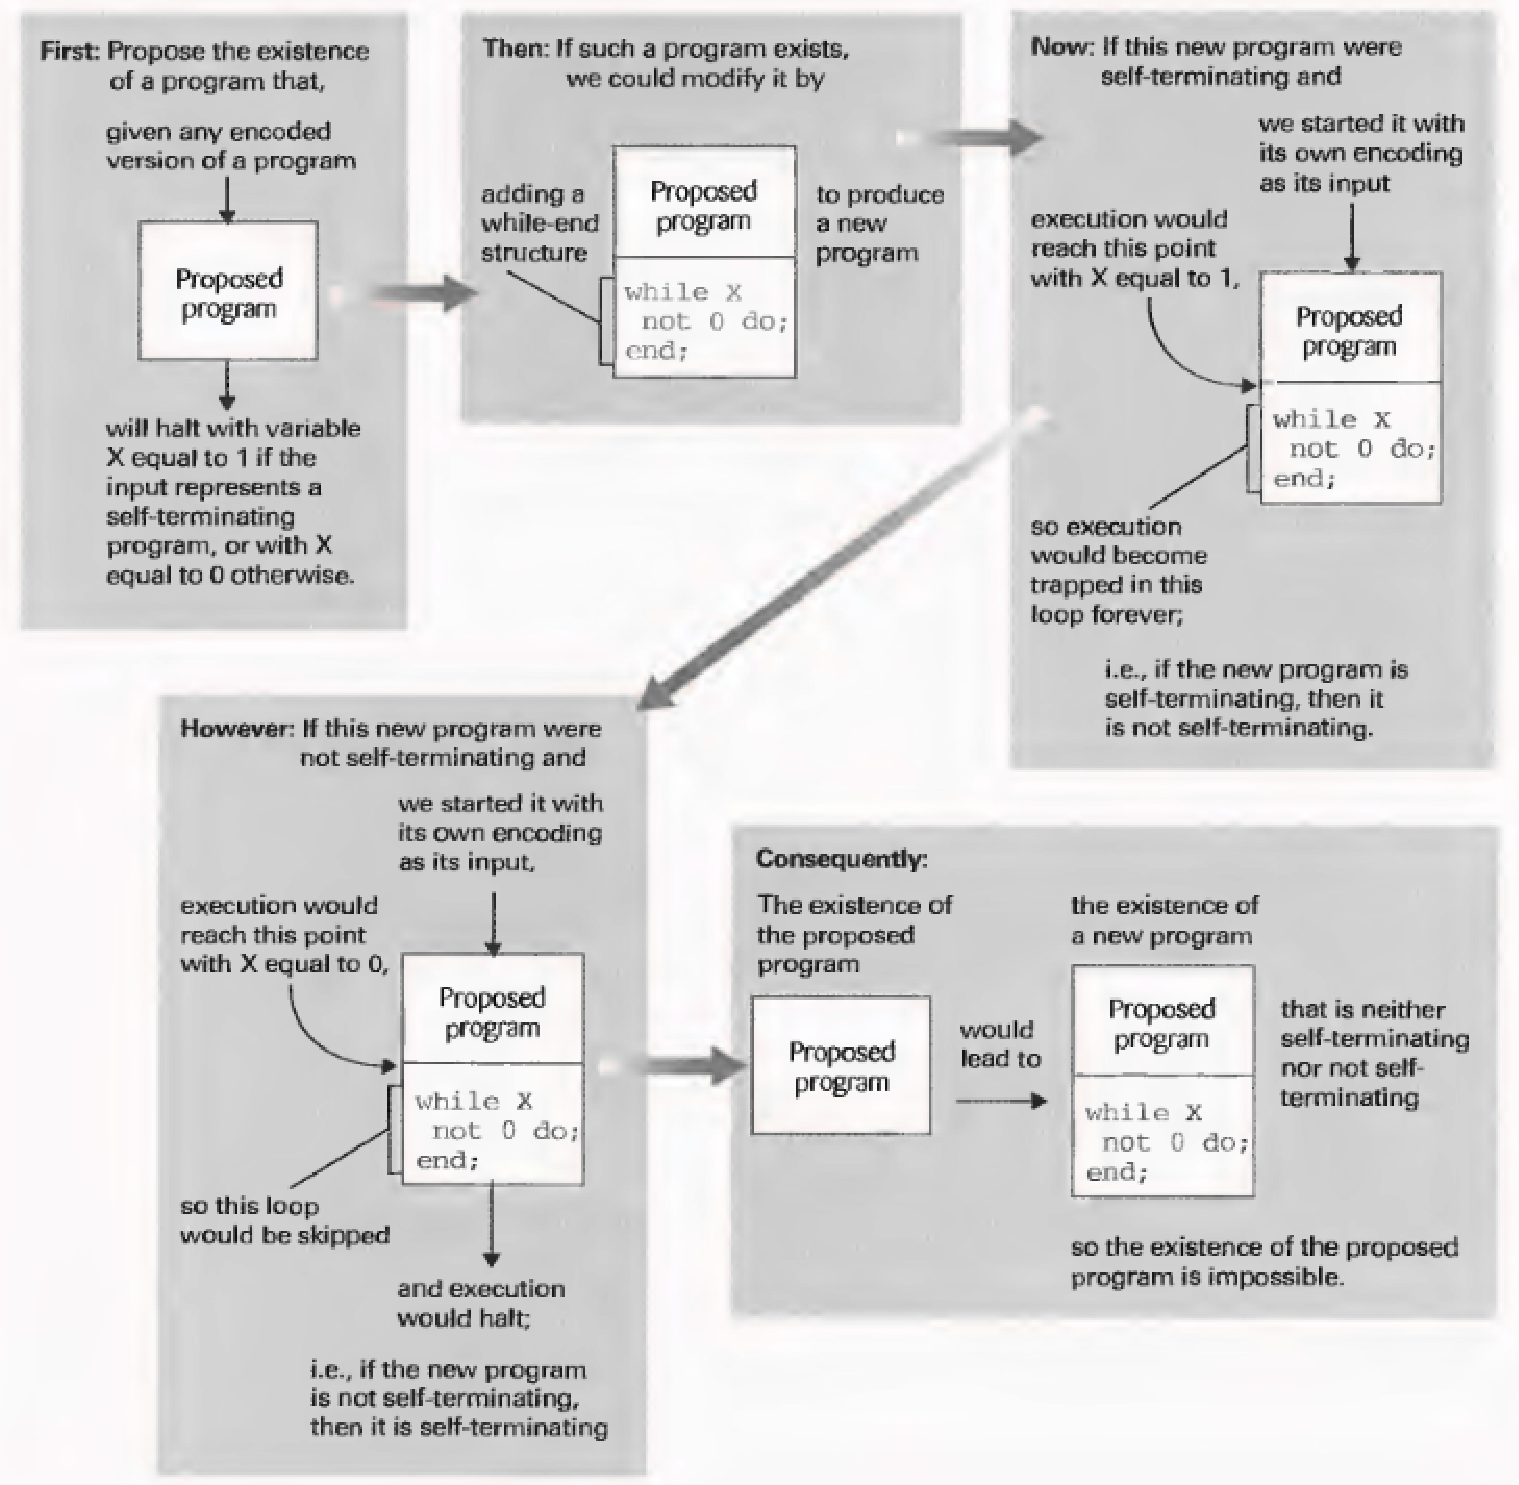
\includegraphics{ch7/fig117.pdf}}
  \caption{Chứng minh tính không giải được của bài toán dừng}
  \label{fig:fig117}
\end{figure}

\newpage

%%% Local Variables: 
%%% mode: latex
%%% TeX-master: "../tindaicuong"
%%% End: 

\section{Độ phức tạp của bài toán}
Trong Mục~\ref{sec:114} ta đã thảo luận về tính giải được của bài toán. Trong mục này ta
quan tâm đến câu hỏi khi nào bài toán giải được có một lời giải chấp nhận được trong thực
tế. Ta sẽ thấy rằng một số bài toán về mặt lý thuyết có thể giải được nhưng quá phức tạp,
nên theo quan điểm thực tế chúng là không giải được.

\subsection*{Đo độ phức tạp của bài toán}

Ta bắt đầu bằng việc xem xét lại các nghiên cứu của ta về tính hiệu quả của thuật toán
trong Mục~\ref{}. Ở đây ta sử dụng ký hiệu theta-lớn để phân loại thuật toán theo thời
gian yêu cầu thực hiện. Ta thấy rằng thuật toán sắp xếp chèn thuộc lớp~$\Theta(n^2)$,
thuật toán tìm kiếm tuần tự là thuộc lớp $\Theta(n)$, và thuật toán tìm kiếm nhị phân
thuộc lớp $\Theta(\lg n)$. Bây giờ ta dùng hệ thống phân loại này để xác định độ phức tạp
của bài toán. Mục đích của ta là phát triển một hệ thống cho phép chỉ ra bài toán nào là
phức tạp hơn bài toán nào và cuối cùng bài toán nào là quá phức tạp đến mức lời giải của
nó vượt ra khỏi khả năng thực tế.

Lý do để ta trình bày nghiên cứu dựa trên hiểu biết về tính hiệu quả của thuật toán là ta
mong muốn đo độ phức tạp của một bài toán theo độ phức tạp của lời giải. Ta xem xét một
bài toán đơn giản là một bài toán có một lời giải đơn giản; một bài toán phức tạp là bài
toán không có lời giải đơn giản. Để ý rằng sự kiện rằng bài toán có một lời giải khó không
có nghĩa rằng bài toán là phức tạp. Bởi vì bài toán đó có thể có nhiều lời giải, một trong
số chúng là phức tạp. Bởi vậy, kết luận rằng một bài toán là phức tạp yêu cầu rằng ta phải
chỉ ra rằng nó không có lời giải nào đơn giản.

Trong khoa học máy tính, các bài toán được quan tâm là các bài toán có thể giải bằng
máy. Các lời giải của bài toán này được thiết lập như các thuật toán. Bởi vậy độ phức tạp
của bài toán được xác định bởi tính chất của thuật toán giải bài toán đó. Chính xác hơn,
ta xem độ phức tạp của một bài toán là độ phức tạp của thuật toán đơn giản nhất để giải bài
toán đó.

Nhưng làm thế nào ta có thể đo độ phức tạp của một thuật toán? Không may, thuật ngữ
\textit{độ phức tạp} có nhiều cách giải thích khác nhau. Một trong số đó là xem xét số các
quyết định và rẽ nhánh trong thuật toán. Theo hướng này, một thuật toán phức tạp là thuật
toán có tập các hướng rẽ nhánh rất lớn. Cách giải thích này phù hợp theo quan điểm của các
kỹ sư phần mềm, những người quan tâm đến đến việc khám phá thuật toán và biểu diễn chúng,
nhưng nó lại không thâu tóm được độ phức tạp theo quan điểm của máy. Máy không thực sự
phải ra quyết định khi lựa chọn lệnh tiếp theo để thực hiện mà nó đơn thuần chỉ thực hiện
theo chu kỳ máy, mỗi lần thực hiện một lệnh được chỉ ra bởi bộ đếm chương trình. Kết quả
là, máy có thể thực hiện một mớ lộn xộn các lệnh cũng dễ như nó thực hiện một danh sách
các lệnh đơn giản tuần tự. Vậy thì, cách giải thích như thế này về độ phức tạp chỉ hướng
tới việc đo mức độ khó khăn gây ra trong một biểu diễn thuật toán hơn là bản thân độ phức
tạp thuật toán.

Một cách giải thích khác phản ánh được chính xác hơn về độ phức tạp của thuật toán từ quan
điểm máy là đo số bước phải thực hiện khi chạy thuật toán. Để ý rằng điều này không đồng
nghĩa với việc tính số lệnh xuất hiện trong chương trình. Một vòng lặp với thân bao gồm
chỉ một lệnh nhưng yêu cầu thực hiện lặp $100$ lần là tương đương với $100$ lệnh khi thực
hiện. Bởi thế lệnh lặp này được xem là phức tạp hơn so với một danh sách~$50$ lệnh đơn, dù
chúng có được viết dài hơn. Vậy thì ý nghĩa của \textit{độ phức tạp} liên quan tới thời
gian máy thực hiện một lời giải chứ không theo kích thước biểu diễn chương trình của lời
giải.

Vậy thì ta xem một bài toán là phức tạp nếu mọi lời giải của nó đều yêu cầu nhiều thời
gian. Định nghĩa về độ phức tạp này thường được gọi là \textbf{độ phức tạp thời gian}. Ta
cũng đã gặp khái niệm độ phức tạp thời gian một cách không trực tiếp trong Mục~\ref{}. Nói
tóm lại, việc nghiên cứu tính hiệu quả của thuật toán chính là nghiên cứu độ phức tạp thời
gian của thuật toán--hai thuật ngữ này có thể dùng thay thế cho nhau. Có nghĩa rằng,
``hiệu quả hơn'' là tương đương với ``ít phức tạp hơn''. Bởi vậy, theo thuật ngữ độ phức
tạp thời gian, thuật toán tìm kiếm tuần tự (ta đã thấy nó là $\Theta(n)$) là một lời giải
phức tạp hơn so với thuật toán tìm kiếm nhị phân (ta đã thấy nó là $\Theta(\lg n)$) cho
bài toán tìm kiếm danh sách .

Ta cùng áp dụng các kiến thức về độ phức tạp thuật toán để tìm ý nghĩa về độ phức tạp của
bài toán. Ta nói độ phức tạp (thời gian) của một bài toán là $\Theta(f(n))$, với~$f(n)$ là
một hàm theo $n$, nếu có một thuật toán để giải quyết bài toán với độ phức tạp thời gian
là $\Theta(f(n))$ và không có thuật toán nào khác có độ phức tạp thời gian thấp hơn. Có
nghĩa rằng độ phức tạp (thời gian) của bài toán được định nghĩa là độ phức tạp (thời gian)
của lời giải tốt nhất. Không may, việc tìm lời giải tốt nhất của một bài toán và biết rằng
nó là tốt nhất lại là một bài toán khó. Trong những tình huống kiểu này, một biến thể của
ký hiệu theta-lớn được gọi là \textbf{ký hiệu O-lớn} (đọc là ``ký hiệu Ô lớn'') được dùng
để biểu diễn những gì ta biết về độ phức tạp của bài toán. Nói chính xác hơn, nếu $f(n)$
là một hàm toán học theo $n$ và nếu bài toán có thể giải bởi một thuật toán trong
$\Theta(f(n))$, vậy thì ta nói rằng bài toán là thuộc vào $O(f(n))$ (đọc là ``Ô lớn
$f(n)$''). Bởi vậy, để nói rằng một bài toán thuộc vào $O(f(n))$ có nghĩa rằng nó có một
lời giải với độ phức tạp là trong~$\Theta(f(n))$ nhưng có thể có một lời giải tốt hơn.

Thảo luận của ta về các thuật toán sắp xếp và tìm kiếm chỉ ra rằng bài toán tìm kiếm trong
một danh sách $n$ phần tử (khi ta đã biết danh sách trước đó đã được sắp) là trong thời
gian $O(\lg n)$ do thuật toán tìm kiếm nhị phân có thể giải bài toán này. Hơn nữa, các nhà
nghiên cứu đã chứng minh rằng bài toán tìm kiếm thực sự là trong $\Theta(\lg n)$, bởi thế
tìm kiếm nhị phân biểu diễn một thuật toán tối ưu cho bài toán này. Ngược lại, ta biết
rằng bài toán sắp xếp một danh sách có $n$ phần tử (khi ta không biết gì về phân phối của
các giá trị bên trong danh sách) là trong $O(n^2)$ do thuật toán sắp xếp chèn có thể giải
bài toán này. Tuy nhiên, bài toán sắp xếp đã được biết là có độ phức tạp trong $\Theta(n
\lg n)$, điều này chỉ ra rằng thuật toán sắp xếp chèn không phải là một lời giải tối ưu
(theo ngữ cảnh độ phức tạp thời gian).

%Thiếu phần sắp xếp chèn
%[... thuật toán sắp xếp chèn ....]
%
\subsection*{Bài toán đa thức và không đa thức}
Giả sử rằng $f(n)$ và $g(n)$ là hai hàm theo $n$. Ta nói rằng $g(n)$ là bị chặn bởi $f(n)$
có nghĩa rằng với giá trị $n$ đủ lớn, giá trị của $f(n)$ sẽ lớn hơn $g(n)$ và vẫn lớn hơn
$g(n)$ với mọi giá trị lớn hơn của $n$ . Nói cách khác, hàm $g(n)$ bị chặn bởi $f(n)$ có
nghĩa rằng đồ thị~$f(n)$ sẽ ở phía trên đồ thị của $g(n)$ với các giá trị của $n$
``lớn''. Ví dụ, hàm $g(n)=\lg n$ là bị chặn bởi hàm $f(n)=n$ (Hình~\ref{fig:fig1111a}), và
hàm $n \lg n$ là bị chặn bởi hàm $n^2$ (Hình~\ref{fig:fig1111b}).

\begin{figure}
\centering
\subfloat[ $n$ và $\lg n$]{
    \scalebox{0.35}{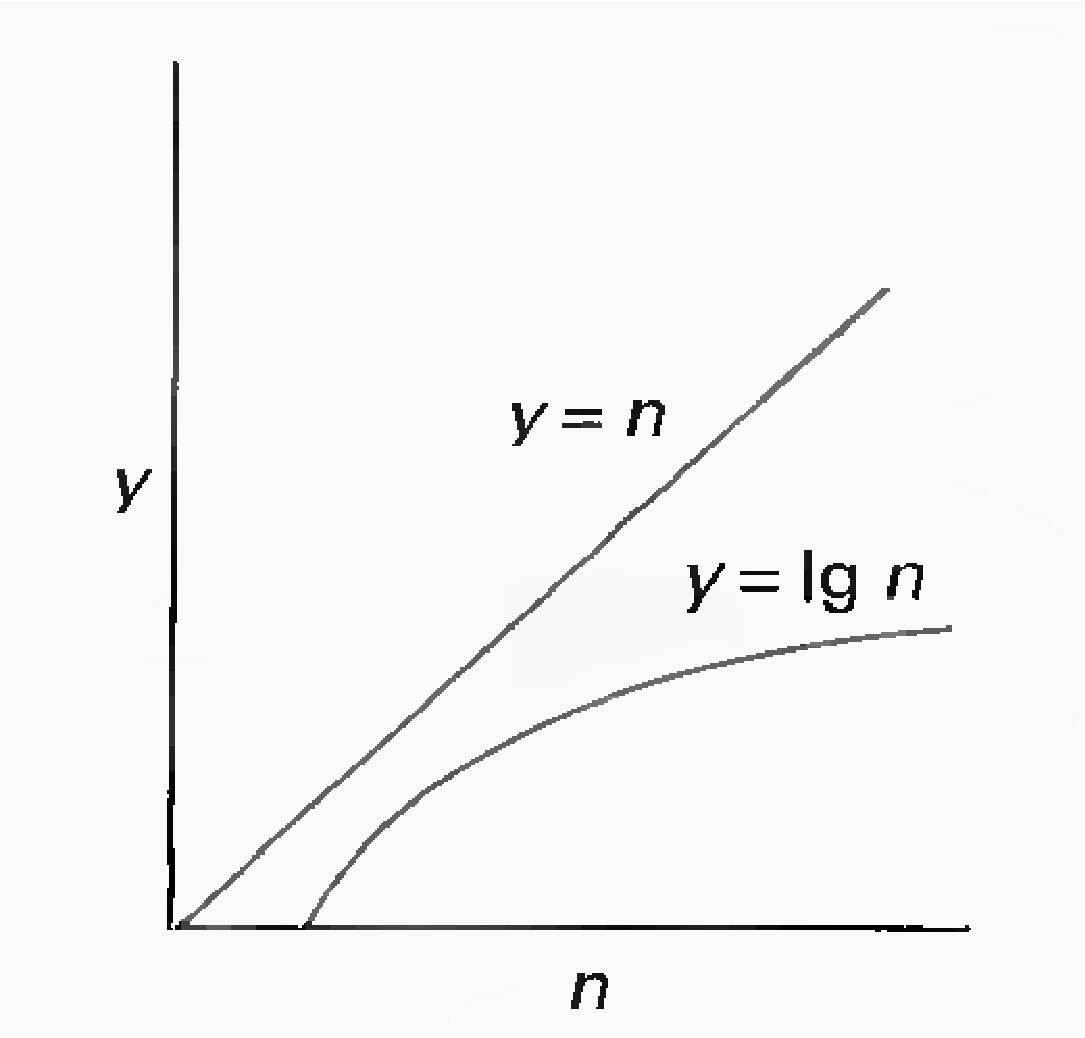
\includegraphics{ch7/fig1111.pdf}}
\label{fig:fig1111a}
}\qquad  \subfloat[ $n^2$ và $n \lg n$]{
  \scalebox{0.35}{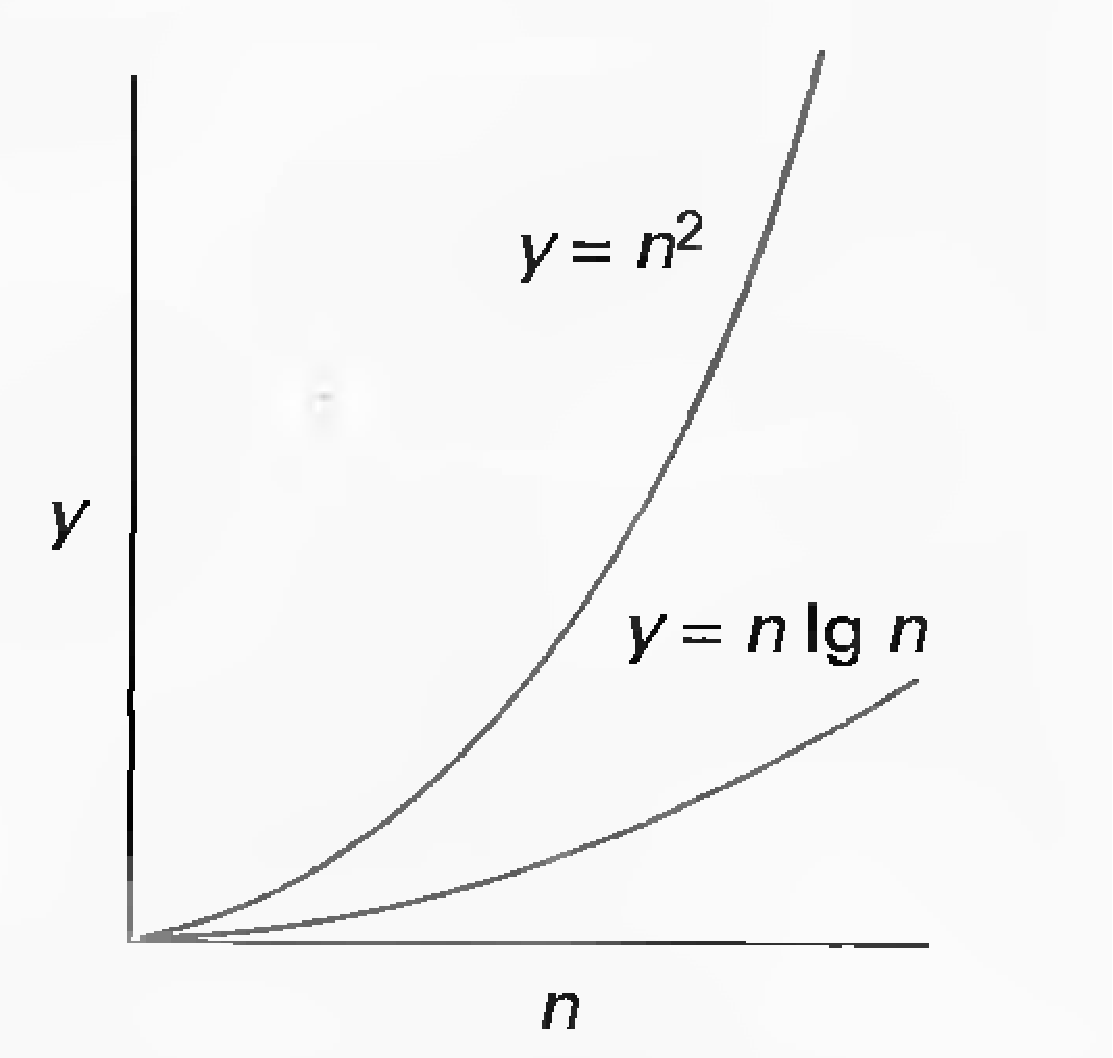
\includegraphics{ch7/fig1111b.pdf}}
\label{fig:fig1111b}
}  
\caption{Đồ thị của các hàm $n, \lg n, n \lg n,$ và $n^2$}
\end{figure}

Ta nói rằng một bài toán là \textbf{bài toán đa thức} nếu bài toán là $O(f(n))$, ở đó hàm
$f(n)$ hoặc là một đa thức hoặc bị chặn bởi một đa thức. Tập mọi bài toán đa thức được
biểu diễn bởi $\mathbf{P}$. Để ý rằng các thảo luận trước của ta chỉ ra rằng các bài toán
tìm kiếm danh sách và sắp xếp danh sách thuộc vào lớp $\mathbf{P}$.

Để nói rằng một bài toán là bài toán đa thức tức là khẳng định về thời gian yêu cầu để
giải bài toán đó. Ta thường nói rằng một bài toán trong $\mathbf{P}$ có thể được giải
trong thời gian đa thức hoặc bài toán có một lời giải trong thời gian đa thức.

Trong khoa học máy tính, việc xác định các bài toán thuộc vào lớp $\mathbf{P}$ là rất quan
trong bởi vì nó liên quan chặt chẽ đến các bài toán có lời giải chấp nhận được trong thực
tế. Thật vậy, các bài toán bên ngoài lớp $\mathbf{P}$ được đặc trưng như các bài toán có
thời gian chạy vô cùng lâu, thậm chí với đầu vào có kích thước nhỏ. Ta xem xét, ví dụ một
bài toán để tìm lời giải cần $2^n$ bước. Hàm $2^n$ rõ ràng không bị chặn bởi đa thức--nếu
$f(n)$ là một đa thức, vậy nếu ta tăng giá trị của $n$, ta sẽ thấy rằng các giá trị $2^n$
cuối cùng sẽ lớn hơn so với $f(n)$. Có nghĩa rằng một thuật toán với độ phức tạp
$\Theta(2^n)$ nói chũng sẽ ít hiệu quả, và bởi vậy nó yêu cầu nhiều thời gian hơn so với
một thuật toán với độ phức tạp $\Theta(f(n))$. Một thuật toán ở đó độ phức tạp là hàm mũ
được gọi là đòi hỏi thời gian mũ.

Ta xét một ví dụ cụ thể, là bài toán liệt kê mọi khả năng phân nhóm từ một tập có~$n$ phần
tử. Bởi vì có $2^n - 1$ cách phân nhóm (ta cho phép một nhóm có đủ tất cả mọi phần tử
nhưng không có phép nhóm không có phần tử nào), mọi thuật toán giải bài toán này cần ít
nhất $2^n - 1$ bước và bởi vậy độ phức tạp của nó ít nhất phải bằng với số này. Nhưng hàm
$2^n -1$ là hàm mũ, vậy nó không bị chặn bởi một đa thức. Bởi vậy mọi lời giải của bài
toán này tiêu tốn lượng thời gian vô cùng lớn nếu số phần tử của tập cần phân nhóm tăng
lên.

Ta thấy rằng bài toán phân nhóm có độ phức tạp lớn là do kích thước của đầu ra lớn. Tuy
nhiên, có tồn tại những bài toán độ phức tạp lớn thậm chí với đầu ra chỉ đơn thuần là câu
trả lời đơn giản có hay không. Một ví dụ là khả năng trả lời một câu hỏi về tính chân thực
của mệnh đề liên quan đến phép cộng các số thực. Ví dụ ta có thể nhận ra rằng câu hỏi ``có
tồn một số thực để tổng của nó với chính nó cho kết quả bằng $6$?'' có câu trả lời là có,
trong khi đó câu trả lời của câu hỏi ``có tồn tại một số thực khác không để tổng của nó
với chính nó bằng $0$?'' là không. Tuy vậy, khi câu hỏi phức tạp lên, ta sẽ gặp rất nhiều
khó khăn nếu muốn trả lời. Và nếu việc đối mặt với nhiều câu hỏi gợi ý cho ta rằng có thể
dùng máy tính để trợ giúp, thì không may, khả năng trả lời câu hỏi này đã được chứng minh
là đòi hỏi thời gian mũ, bởi thế, máy tính cuối cùng sẽ không thể trả lời câu hỏi này
trong thời gian cho phép khi câu hỏi phức tạp hơn.

Sự thật rằng các bài toán có thể giải được về mặt lý thuyết nhưng không ở
trong~$\mathbf{P}$ là có độ phức tạp thời gian vô cùng lớn đưa ta đến kết luận rằng các
bài toán này về cơ bản là không giải được trên thực tế. Các nhà khoa học máy tính gọi
chúng là các \textbf{bài toán bất trị}. Nói tóm lại, lớp $\mathbf{P}$ là một biên giới để
phân định bài toán nào là bất trị theo quan điểm thực tế. Bởi vậy nghiên cứu lớp
$\mathbf{P}$ là rất quan trọng đối với khoa học máy tính.

\subsection*{Bài toán NP}
Ta cùng xem xét \textbf{bài toán người bán hàng du lịch} (Travelling Salesman Problem, gọi
tắt là TSP). Yêu cầu của bài toán này là người bán hàng du lịch phải đi đến thăm từng
khách hàng của ở các thành phố khác nhau mà không được vượt quá ngân sách cho phép. Vấn đề
của anh ta là phải tìm một đường đi (bắt đầu từ nhà, đến các thành phố yêu cầu, rồi quay
về nhà) với độ dài đường đi không vượt quá số kilômét cho phép.

Lời giải cổ điển của bài toán này là xem xét một cách có hệ thống mọi đường đi có thể, và
so sánh độ dài của mỗi đường đi với số kilômét giới hạn cho tới khi tìm thấy một đường đi
chấp nhận được hoặc đã xem xét mọi khả năng. Cách tiếp cận này, tuy vậy không cho một lời
giải trong thời gian đa thức. Điều này là do khi số thành phố tăng lên, số các đường đi
phải kiểm tra tăng lên nhanh hơn so với mọi đa thức. Bởi vậy, việc giải bài toán TSP theo
cách này là không thực tế trong trường hợp số thành phố lớn.

Vậy muốn giải bài toán TSP trong thời gian chấp nhận được ta cần phải tìm một thuật toán
nhanh hơn. Giải pháp tham lam của ta là quan sát xem có một đường đi nào thoả mãn và sau
đó xem chuyện gì xảy ra nếu ta lựa chọn nó. Thuật toán này kết thúc rất nhanh chóng. Cụ
thể, danh sách các lệnh dưới đây có thể thực hiện nhanh chóng và có khả năng giải bài toán
này:
\begin{flushleft}
  \qquad     \textsl{Lấy một đường đi có thể, và tính toán khoảng cách của nó.} \\
  \qquad    \textsl{\textbf{If} (khoảng cách này không lớn hơn số kilômét cho phép)} \\
  \qquad    \textsl{\textbf{then} (thông báo thành công)} \\
  \qquad \textsl{\textbf{else} (thông báo không có)}
\end{flushleft}
Tuy nhiên, về mặt kỹ thuật dãy lệnh này không phải là một thuật toán. Lệnh đầu tiên là
nhập nhằng và ta không thể xác định đường đi nào được chọn hay không được chọn, và cũng
không xác định được làm thế nào có thể ra quyết định chọn. Thay vào đó nó cần đến sự sáng
tạo của cơ chế thực hiện chương trình để ra quyết định. Ta nói rằng các lệnh kiểu này là
không đơn định, và ta gọi một ``thuật toán'' chứa các lệnh kiểu này là \textbf{thuật toán
  không đơn định}.

Để ý rằng khi số các thành phố tăng lên, thời gian cần để thực hiện thuật toán không đơn
định ở trên tăng một cách chậm chạp. Quá trình lựa chọn một đường đi chỉ đơn thuần là đưa
ra một danh sách các thành phố, điều này có thể được làm trong khoảng thời gian tỉ lệ với
số các thành phố được yêu cầu. Hơn nữa, thời gian yêu cầu tính toán tổng khoảng cách trên
đường đi được chọn cũng tỉ lệ với số các thành phố được thăm, và thời gian yêu cầu để so
sánh tổng này với số kilômét giới hạn là độc lập với số thành phố. Nói tóm lại, thời gian
yêu cầu thực hiện thuật toán không đơn định này bị chặn bởi một đa thức. Bởi vậy ta có thể
giải bài toán TSP bởi một thuật toán không đơn định trong thời gian đa thức.

Tất nhiên, lời giải không đơn định của ta không thoả mãn về mặt tổng thể. Nó cần đến một
sự ước đoán may mắn. Nhưng sự tồn tại của nó lại gợi ý cho ta rằng có thể có một lời giải
đơn định của bài toán này chạy trong thời gian đa thức. Vấn đề thực sự có hay không một
thuật toán như vậy đến nay vẫn là một câu hỏi mở. Thực ra, bài toán TSP là một trong nhiều
bài toán được biết là có lời giải không đơn định chạy trong thời gian đa thức nhưng chưa
tìm thấy lời giải đơn định trong thời gian đa thức. Lời giải không đơn định trong thời
gian đa thức này làm ta hy vọng rằng một ngày nào đó sẽ tìm thấy một lời giải hiệu quả
thời gian đa thức. Tuy vậy, đến nay hầu hết mọi người đều tin rằng các bài toán kiểu này
là đủ phức tạp vượt ra ngoài khả năng của các thuật toán đơn định hiệu quả.

Bài toán có thể được giải trong thời gian đa thức bởi một thuật toán không đơn định được
gọi là một \textbf{bài toán đa thức không đơn định}, hay gọi tắt là \textbf{bài toán
  NP}. Ta thường ký hiệu lớp bài toán NP bằng $\mathbf{NP}$. Để ý rằng mọi bài toán trong
lớp $\mathbf{P}$ cũng thuộc $\mathbf{NP}$, bởi vì mọi thuật toán (đơn định) có thể thêm
một lệnh không đơn định vào mà không ảnh hưởng đến hiệu quả của chúng.

Tuy vậy câu hỏi có phải mọi bài toán NP cũng thuộc P vẫn là câu hỏi mở, như được chỉ ra
bởi bài toán TSP. Đây là bài toán chưa giải được nổi tiếng nhất trong khoa học máy tính
ngày nay. Lời giải của nó có rất nhiều ý nghĩa thực tế.

Trong nỗ lực giải quyết câu hỏi xem lớp $\mathbf{NP}$ có bằng $\mathbf{P}$ hay không,
người ta đã tìm thấy một lớp bài toán đặc biệt thuộc lớp $\mathbf{NP}$ gọi là các
\textbf{bài toán NP đầy đủ}. Các bài toán này có tính chất là nếu có một thuật toán thời
gian đa thức để giải một trong những bài toán này, thì sẽ có một thuật toán đơn định thời
gian đa thức để giải mọi bài toán khác trong lớp $\mathbf{NP}$; và vậy thì, lớp
$\mathbf{NP}$ trùng với lớp $\mathbf{P}$. Bài toán TSP là một ví dụ của một bài toán NP
đầy đủ.

\begin{figure}
  \centering
    \scalebox{0.3}{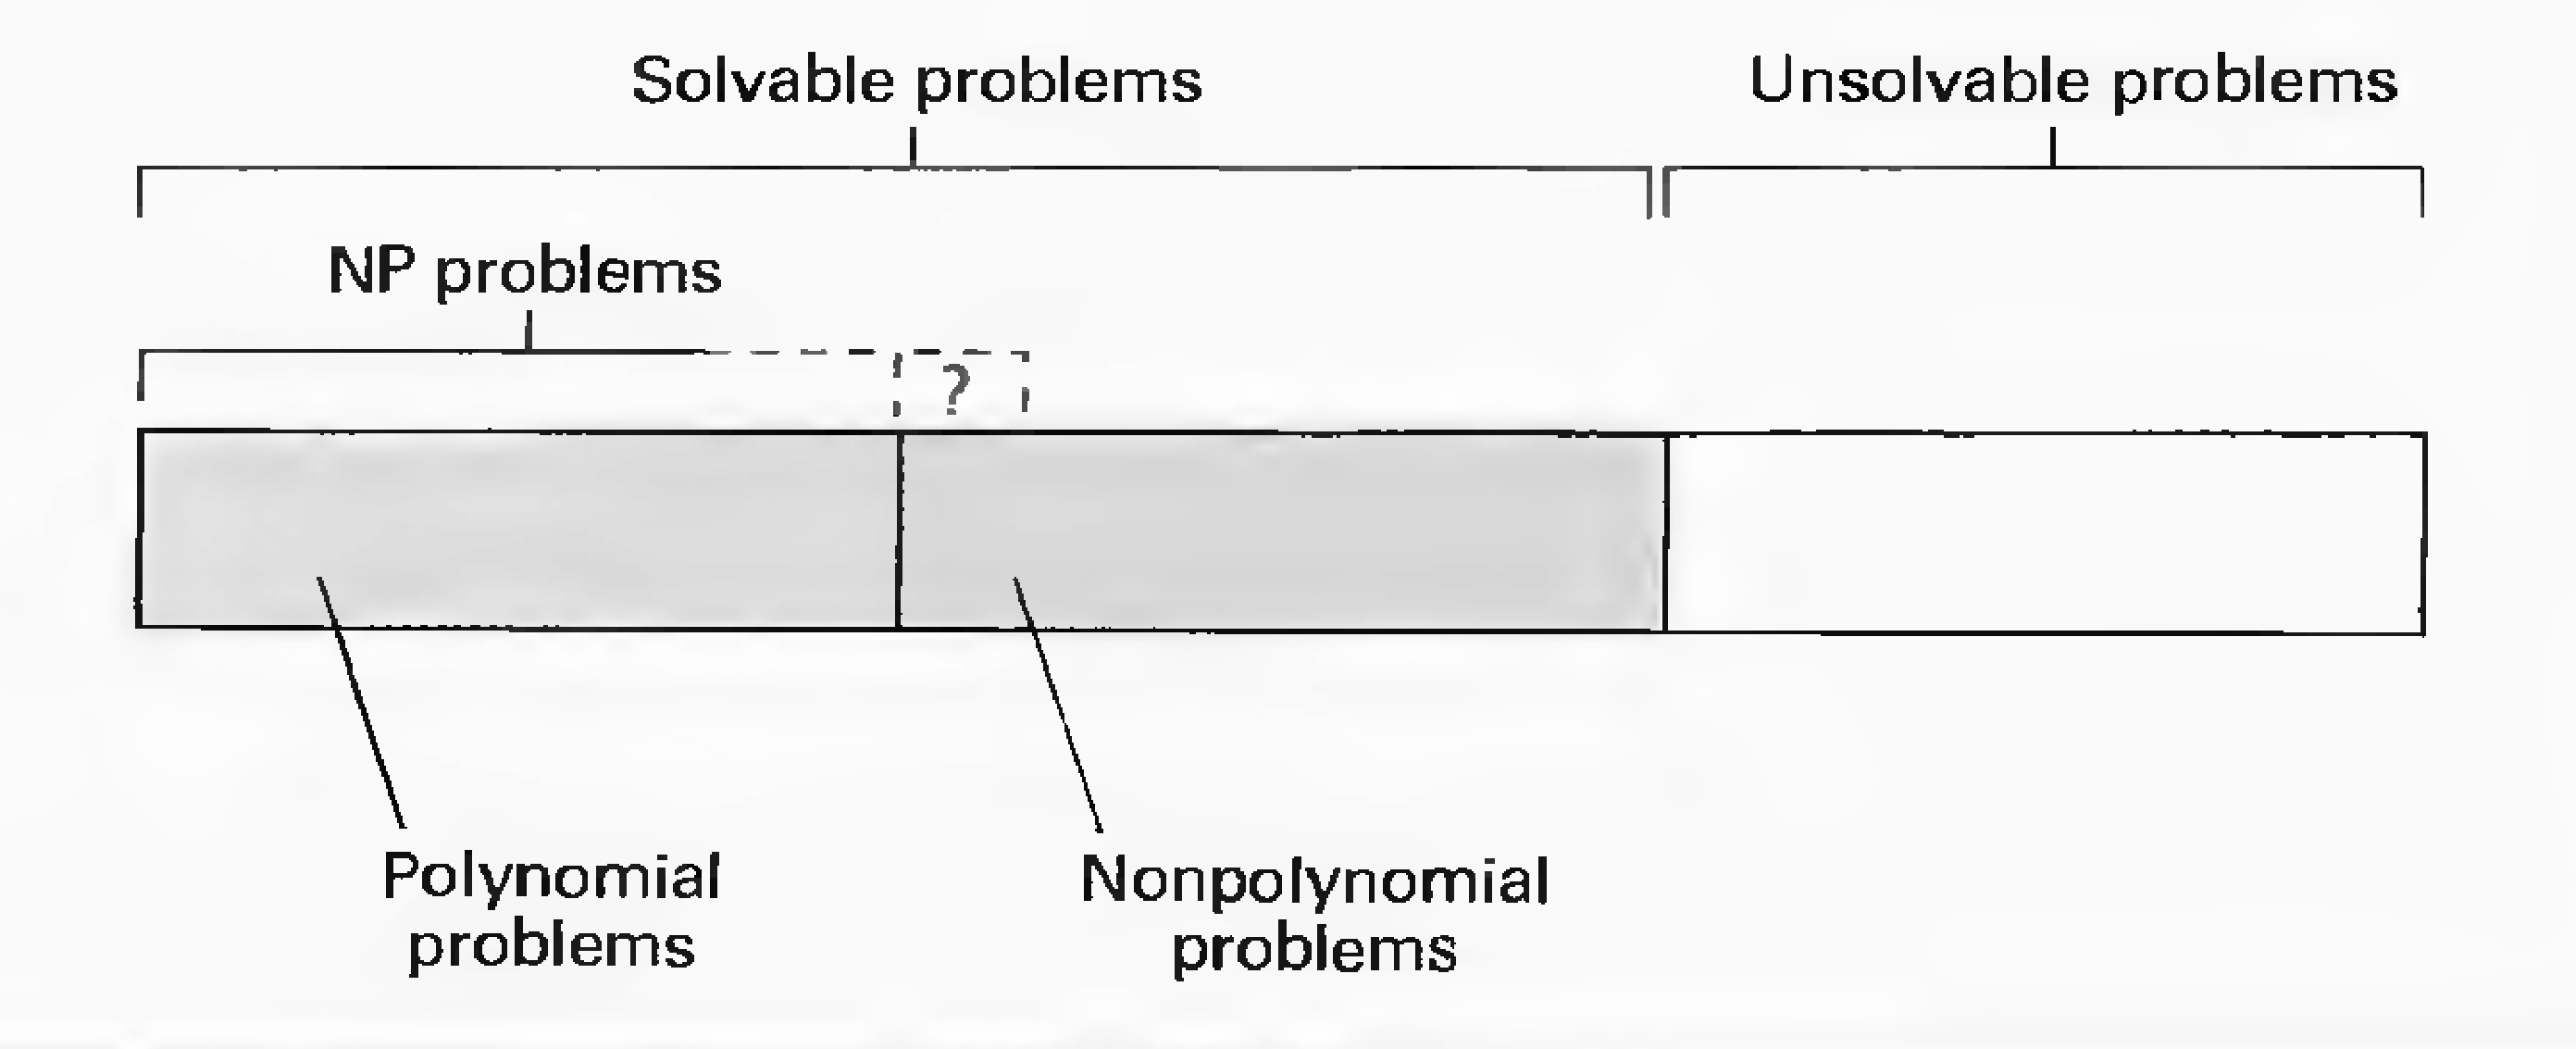
\includegraphics{ch7/fig1112.pdf}}
  \caption{Phân loại các lớp bài toán}
  \label{fig:fig1112}
\end{figure}

Tóm lại, một bài toán có thể phân loại thành hoặc giải được (có lời giải thuật toán) hoặc
không giải được (không có lời giải thuật toán), như được chỉ ra trong
Hình~\ref{fig:fig1112}. Hơn nữa, lớp các bài toán giải được lại được chia thành hai lớp
con. Một là lớp các bài toán thời gian đa thức, bao gồm các bài toán có lời giải chấp nhận
được trong thực tế. Hai là lớp các bài toán không đa thức, với các bài toán này lời giải
chấp nhận trong thực tế của chúng bị giới hạn với các đầu vào kích thước nhỏ và được lựa
chọn cẩn thận. Cuối cùng là lớp bài toán NP bí ẩn mà với hiểu biết hiện tại ta vẫn chưa
thể phân loại được.


\subsection*{Câu hỏi \& Bài tập}

\begin{enumerate}
\item Giả sử rằng một bài toán có thể giải được bởi một thuật toán trong $\Theta(2^n)$. Vậy
  ta có kết luận gì về độ phức tạp của bài toán này?

\item Giải sử một bài toán có thể được giải bởi một thuật toán trong $\Theta(n^2)$ và một
  thuật toán khác trong $\Theta(2^n)$. Thuật toán nào sẽ thực hiện tốt hơn?


\item Liệt kê mọi cách phân nhóm từ tập hai thành viên: Alice và Bill. Liệt kê mọi cách
  phân nhóm tập ba thành viên: Alice, Bill, và Carol. Liệt kê mọi cách phân nhóm của tập
  bốn thành viên: Alice, Bill, Carol, và David.


\item Hãy đưa ra một ví dụ về bài toán đa thức. Đưa ra một ví dụ về bài toán không đa
  thức. Đưa ra một ví dụ của về bài toán NP và chưa được chứng minh là bài toán đa thức.


\item Nếu độ phức tạp của thuật toán \texttt{X} lớn hơn độ phức tạp của thuật toán
  \texttt{Y}, có nhất thiết thuật toán \texttt{X} là khó hiểu hơn thuật toán \texttt{Y}?
  Hãy giải thích câu trả lời của bạn.
\end{enumerate}





%%% Local Variables: 
%%% mode: latex
%%% TeX-master: "../tindaicuong"
%%% End: 

\section{Bài tập cuối chương}
  

\begin{multicols}{2}
  \begin{enumerate}

  \item Chỉ ra xem làm thế nào cấu trúc có dạng:
    \begin{flushleft}
      \quad\texttt{while X equals 0 do;} \\
      \quad\quad \texttt{.} \\
      \quad\quad \texttt{.} \\
      \quad\quad \texttt{.} \\
      \quad\texttt{end;}
    \end{flushleft}
    có thể được mô phỏng với Bare~Bones.

  \item Viết một chương trình Bare~Bones đặt giá trị $1$ vào biến \texttt{Z} nếu biến
    \texttt{X} nhỏ hơn hoặc bằng biến \texttt{Y}, ngược lại đặt giá trị $0$ vào biến
    \texttt{Z}.

  \item Viết một chương trình Bare~Bones đặt \texttt{X} lần giá trị $2$ (hay $2^X$) vào
    biến~\texttt{Z}.

  \item Trong mỗi trường hợp sau đây hãy viết một đoạn chương trình Bare~Bones thực hiện
    các việc được chỉ ra dưới đây:
    \begin{enumerate}
    \item Gán \texttt{Z} bằng $0$ nếu \texttt{X} là số chẵn; ngược lại gán \texttt{Z} bằng
      $1$.

    \item Tính tổng các số nguyên từ $0$ đến \texttt{X}.
    \end{enumerate}


  \item Viết một đoạn chương trình Bare~Bones chia giá trị \texttt{X} cho giá trị
    \texttt{Y}. Ta quy ước bỏ qua phần dư; có nghĩa rằng, $1$ chia $2$ bằng $0$ và $5$
    chia~$3$ bằng $1$.

  \item Mô tả hàm tính bởi chương trình Bare~Bones dưới đây, với giả sử đầu vào biểu diễn
    bởi \texttt{X} và \texttt{Y}; còn đầu ra biểu diễn bởi bởi \texttt{Z}:
    \begin{flushleft}
      \quad\texttt{copy X to Z;} \\
      \quad\texttt{copy Y to Aux;} \\
      \quad\texttt{while Aux not 0 do;} \\
      \quad\quad \texttt{decr Z} \\
      \quad\quad \texttt{decr Aux} \\
      \quad\texttt{end;}
    \end{flushleft}

  \item Mô tả hàm tính bởi chương trình Bare~Bones dưới đây, với giả sử đầu vào biểu diễn
    bởi \texttt{X} và \texttt{Y}; còn đầu ra biểu diễn bởi bởi \texttt{Z}:
    \begin{flushleft}
      \quad\texttt{clear Z;} \\
      \quad\texttt{copy X to Aux1;} \\
      \quad\texttt{copy Y to Aux2;} \\
      \quad\texttt{while Aux1 not 0 do;} \\
      \quad \quad\texttt{while Aux2 not 0 do;} \\
      \quad \quad\quad \texttt{decr Z} \\
      \quad \quad\quad \texttt{decr Aux2} \\
      \quad \quad\texttt{end;} \\
      \quad \quad \texttt{decr Aux1;} \\
      \quad\texttt{end;} \\
    \end{flushleft}

  \item Viết một chương trình Bare~Bones tính tuyển loại của hai biến \texttt{X} và
    \texttt{Y}, đặt kết quả vào biến \texttt{Z}. Giả sử rằng~\texttt{X} và~\texttt{Y} khởi
    tạo với giá trị chỉ bằng~$0$ hoặc~$1$.

  \item Chỉ ra rằng nếu ta cho phép các lệnh trong Bare~Bones được gán nhãn bởi một giá
    trị nguyên và thay thế cấu trúc lặp \texttt{while} với lệnh nhảy điều kiện biểu diễn
    dưới dạng
    \begin{flushleft}
      \texttt{if \textit{tên} not 0 goto \textit{nhãn};}
    \end{flushleft}
    với \texttt{\it tên} có thể là mọi biến và \texttt{\it nhãn} là một giá trị nguyên
    được sử dụng để gán cho một lệnh nào đó, thì ngôn ngữ mới vẫn là ngôn ngữ lập
    trình phổ dụng.

  \item Trong chương này ta đã thấy cách cài đặt lệnh
    \begin{flushleft}
      \texttt{copy \textit{tên1} to \textit{tên2};}
    \end{flushleft}
    trong Bare~Bones. Chỉ ra xem làm thế nào lệnh này có thể được cài đặt nếu cấu trúc
    \texttt{while} được thay thế bởi cấu trúc lặp sau
    \begin{flushleft}
      \texttt{repeat \dots until (\textit{tên} equals 0)}
    \end{flushleft}

  \item Chỉ ra rằng ngôn ngữ Bare~Bones có thể vẫn là ngôn ngữ lập trình phổ dụng nếu lệnh
    \texttt{while} được thay thế bởi cấu trúc lặp sau 
    \begin{flushleft}
      \texttt{repeat \dots until (\textit{tên} equals 0)}
    \end{flushleft}

  \item Thiết kế một máy Turing chỉ dùng duy nhất một ô trên băng nhưng nó không bao giờ
    đạt được trạng thái dừng.

  \item Thiết kế một máy Turing đặt các số~$0$ vào mọi ô bên trái của ô nhớ hiện thời cho
    tới khi nó gặp một ô nhớ chứa dấu sao.

  \item Giả sử xâu gồm các số $0$ và $1$ trên băng của một máy Turing được giới hạn bởi
    các dấu sao ở hai đầu. Thiết kế một máy Turing quay xâu bít này sang phải một ô, giả
    sử rằng máy bắt đầu với ô nhớ hiện hành chứa dấu sao bên phải nhất của xâu.

  \item Thiết kế một máy Turing đảo xâu bít~$0$ và $1$ nằm giữa ô nhớ hiện hành (có chứa
    dấu sao) và ô nhớ chứa dấu sao đầu tiên bên trái.

  \item Tóm tắt luận đề Church-Turing.

  \item Chương trình Bare~Bones sau đây có tự kết thúc? Giải thích câu trả lời của bạn
    \begin{flushleft}
      \texttt{copy X to Y;} \\
      \texttt{incr Y;} \\
      \texttt{incr Y;} \\
      \texttt{while X not 0 do;} \\
      \quad \texttt{decr X;} \\
      \quad \texttt{decr X;} \\
      \quad \texttt{decr Y;} \\
      \quad \texttt{decr Y;} \\
      \texttt{end;}\\
      \texttt{decr Y;} \\
      \texttt{while Y not 0 do;} \\
      \quad \texttt{incr X;} \\
      \quad \texttt{decr Y;} \\
      \texttt{end;}\\
      \texttt{while X not 0 do;}\\
      \texttt{end;}\\
    \end{flushleft}


  \item Chương trình Bare~Bones sau đây có tự kết thúc? Giải thích câu trả lời của bạn.
    \begin{flushleft}
      \texttt{while X not 0 do;}\\
      \texttt{end;}\\
    \end{flushleft}

  \item Chương trình Bare~Bones sau đây có tự kết thúc? Giải thích câu trả lời của bạn.
    \begin{flushleft}
      \texttt{while X not 0 do;}\\
      \quad \texttt{decr X;}\\
      \texttt{end;}\\
    \end{flushleft}

  \item Phân tích tính hợp lệ của cặp lệnh sau đây:
    \begin{flushleft}
      \texttt{Lệnh sau là đúng.}\\
      \texttt{Lênh trước là sai.}\\
    \end{flushleft}

  \item Phân tích tính hợp lệ của khẳng định ``Người đầu bếp trên một con tàu nấu ăn cho
    mọi người và chỉ những những người không nấu được cho bản thân anh ta.'' (Ai nấu ăn
    cho người đầu bếp?)

  \item Giả sử rằng bạn ở trong một thành phố mà mỗi người hoặc là kẻ nói thật, hoặc là kẻ
    nói dối. (Một người nói thật luôn nói sự thật, một người nói dối luôn nói dối.) Bạn có
    thể dùng câu hỏi gì để hỏi một người và biết anh ta là nói thật hay nói dối?

  \item Tóm tắt ý nghĩa của các máy Turing trong lý thuyết khoa học máy tính.

  \item Tóm tắt ý nghĩa của bài toán dừng trong lý thuyết khoa học máy tính.

  \item Giả sử rằng bạn cần phải tìm ra xem có ai trong nhóm của đã sinh vào một ngày đặc
    biệt nào đó. Một cách tiếp cận là có thể hỏi các thành viên vào một lúc nào đó. Nếu
    bạn theo cách tiếp cận này, sự xuất hiện của sự kiện nào có thể chỉ ra cho bạn rằng có
    một thành viên như vậy? Sự kiện nào có thể chỉ cho bạn rằng không có thành viên nào
    như vậy? Bây giờ giả sử rằng bạn phải tìm ra xem có ít nhất một số nguyên dương có
    tính chất đặc biệt nào đó và bạn áp dụng cùng cách tiếp cận kiểm tra một cách có hệ
    thống các số nguyên cùng một lúc. Nếu, trên thực tế, có nhiều số nguyên có tính chất
    này, làm thế nào bạn có thể tìm ra? Nếu, tuy vậy, không có số nguyên nào có tính chất
    này làm thế nào bạn có thể tìm ra? Có phải nhiệm vụ kiểm tra xem một giả thuyết là
    đúng có nhất thiết đối xứng với nhiệm vụ kiểm tra xem nó có sai hay không?


  \item Có phải bài toán tìm kiếm một giá trị đặc biệt trong danh sách là bài toán đa
    thức? Chứng minh câu trả lời của bạn.

  \item Thiết kế một thuật toán quyết định xem một số nguyên có là nguyên tố hay không. Có
    phải lời giải của bạn là hiệu quả? Lời giải của bạn là trong thời gian đa thức hay
    không?

  \item Có phải một lời giải đa thức cho một bài toán luôn tốt hơn so với một lời giải mũ?
    Giải thích câu trả lời của bạn.

  \item Có phải một bài toán có một lời giải đa thức có nghĩa rằng nó luôn được giải trong
    thời gian có thể chấp nhận trong thực tế? Giải thích câu trả lời của bạn.


  \item Lập trình viên Charlie được giao bài toán phân nhóm (của một số chẵn người) vào
    thành hai nhóm con rời nhau và có số người bằng nhau sao cho sự khác biệt về tuổi của
    mỗi nhóm con là lớn nhất có thể. Anh ta đề nghị một lời giải là liệt kê mọi khả năng
    chia thành hai nhóm, tính toán sự khác biệt về tuổi của mỗi cặp, và lựa chọn ra cặp
    nhóm có khác biệt nhiều nhất. Lập trình viên Mary có một giải pháp khác, chị đề nghị
    rằng đầu tiên sắp xếp nhóm ban đầu theo tuổi và sau đó chia thành hai nhóm con. Mỗi
    nhóm con gồm một nửa từ nửa những người trẻ hơn và nửa còn lại từ những người già
    hơn. Hãy chỉ ra độ phức tạp của mỗi lời giải? Có phải bài toán này có độ phức tạp là
    đa thức, $\mathbf{NP}$, hay không đa thức?

  \item Tại sao cách tiếp cận sinh mọi khả năng có thể sắp xếp danh sách sau đó chọn một
    cách sắp xếp mong muốn không phải là cách hợp lý để sắp xếp một danh sách?

  \item Giả sử trò chơi xổ số dựa trên việc chọn đúng bốn số nguyên, mỗi số trong khoảng
    từ $1$ đến $50$. Hơn nữa giả sử rằng giải thưởng là quá lớn đến mức mà người mua sẽ có
    lợi nếu anh ta mua một vé số riêng cho mỗi tổ hợp số. Nếu bạn mất một giây để mua một
    vé, bạn sẽ mất bao lâu để mua một vé cho mỗi tổ hợp số? Thời gian này sẽ thay đổi thế
    nào nếu công ty xổ số yêu cầu chọn năm số thay vì bốn? bài toán này phải làm gì với
    kiến thức trong chương này?

  \item Thuật toán dưới đây có đơn định không?
    \begin{description}
    \item [] \textsl{\textbf{procedure} mystery (Number)} 

    \item []\textsl{\textbf{if} (Number > 5)} 

    \item[] \textsl{\textbf{then} (trả lời ``yes'')} 

    \item [] \textsl{\textbf{else} (lấy một giá trị nhỏ hơn $5$ và đưa số này ra làm câu
        trả lời)}
    \end{description}

  \item Thuật toán dưới đây có đơn định không? Hãy giải thích câu trả lời của bạn.
    \begin{description}
    \item []\textsl{Lái xe đi thẳng.}

    \item [] \textsl{Đến chỗ đường giao thứ ba, hỏi người đứng ở góc đường xem nên rẽ phải
        hay rẽ trái.}

    \item[] \textsl{Rẽ theo hướng người đó chỉ.}

    \item []\textsl{Lái xe qua thêm hai khối nhà và dừng ở đó.}
    \end{description}

  \item Xác định các điểm không đơn định trong thuật toán sau:
    \begin{description}
    \item []\textsl{Chọn ba số giữa $10$ và $100$.}

    \item [] \textsl{\textbf{if} (tổng của số được chọn lớn hơn~$150$)}

    \item[] \textsl{\textbf{then} (trả lời ``yes'')}

    \item []\textsl{\textbf{else} (Chọn một trong ba số đã chọn và đưa ra số ngày như câu
        trả lời)}
    \end{description}

  \item Thuật toán sau đây có độ phức tạp đa thức hay không đa thức? Giải thích câu trả
    lời của bạn.
    \begin{description}
    \item []\textsl{\textbf{procedure} mystery (ListOfNumbers)}

    \item [] \textsl{Chọn một tập các số trong ListOfNumbers.}

    \item[] \textsl{\textbf{if} (các số trong tập này cộng thêm với $125$)}

    \item []\textsl{\textbf{then} (Câu trả lời ``yes'')}

    \item []\textsl{\textbf{else} (Không đưa ra câu trả lời)}

    \end{description}

  \item Các bài toán dưới đây có thuộc lớp~$\mathbf{P}$?
    \begin{enumerate}
    \item Một bài toán với độ phức tạp~$n^2$

    \item Một bài toán với độ phức tạp~$3n$

    \item Một bài toán với độ phức tạp~$n^2 + 2n$

    \item Một bài toán với độ phức tạp~$n!$
    \end{enumerate}

  \item Tóm tắt sự phân biệt giữa khẳng định một bài toán là bài toán đa thức và khẳng
    định một bài toán là bài toán đa thức không đơn định.

  \item Đưa ra một ví dụ về bài toán thuộc cả lớp $\mathbf{P}$ và $\mathbf{NP}$.

  \item Giả sử rằng bạn được đưa ra hai thuật toán để giải cùng một bài toán. Một thuật
    toán có độ phức tạp thời gian~$n^4$ và một thuật toán có độ phức tạp~$4n$. Với kích
    thước đầu vào như thế nào thì thuật toán đầu hiệu quả hơn thuật toán sau?

  \item Giả sử rằng bạn phải đối mặt với bài toán người bán hàng du lịch trong trường hợp
    số thành phố là $15$ trong đó giữa mọi cặp thành phố đều nối trực tiếp với nhau bởi
    một con đường duy nhất. Có bao nhiêu đường đi khác nhau có thể có đi qua các thành phố
    này? Ta mất bao lâu để tính độ dài của mọi đường đi này biết rằng việc tính độ dài của
    một đường đi mất một micro-giây?

  \item Hãy đưa ra một ví dụ cho mỗi bài toán thuộc một phạm vi biểu diễn trong
    Hình~\ref{fig:fig1112}.

  \item Thiết kế một thuật toán tìm nghiệm nguyên của phương trình có dạng $x^2 + y^2 =
    n$, với $n$ là một số nguyên được đưa vào. Xác định độ phức tạp thời gian thuật toán
    của bạn.

  \item \label{ex:1145} Một bài toán khác cũng thuộc lớp NP đầy đủ là \textbf{bài toán
      sắp ba lô} (Knapsack problem). Bài toán này yêu cầu tìm các số trong danh sách sao
    cho tổng của các số này bằng một giá trị đặc biệt. Ví dụ, ba số $257, 388$ và~$782$
    trong danh sách
    \[
    642, 257, 771, 388, 391, 782, 304
    \]
    có tổng là $1427$. Hãy tìm các số trong danh sách sao cho tổng của chúng là
    $1723$. Bạn áp dụng thuật toán nào? và độ phức tạp của nó là gì?

  \item Hãy xác định điểm tương đồng giữa bài toán người bán hàng du lịch và bài toán sắp
    ba lô (xem bài tập~\ref{ex:1145}).
  \end{enumerate}

  
\end{multicols}


%%% Local Variables: 
%%% mode: latex
%%% TeX-master: "../tindaicuong"
%%% End: 



%%% Local Variables: 
%%% mode: latex
%%% TeX-master: "../tindaicuong"
%%% End: 
